% Classe do documento e parâmetros gerais.
\documentclass[a4paper,openright,twoside,11pt]{report}

% Packages utilizadas e respetivos parâmetros.
\usepackage[utf8]{inputenc}
\usepackage[portuguese]{babel}
\addto{\captionsportuguese}{\renewcommand{\bibname}{Refer\^{e}ncias}}
\addto{\captionsportuguese}{\renewcommand{\contentsname}{\'{I}ndice}}
\addto{\captionsportuguese}{\renewcommand{\appendixname}{Ap\^{e}ndice}}

\usepackage{lipsum} % gerador de texto
\usepackage{graphicx}
\usepackage{url}
\usepackage[Algoritmo]{algorithm}
\usepackage{algorithmicx}
\usepackage{algpseudocode}
\renewcommand{\algorithmicrequire}{\textbf{Dados: }}
\renewcommand{\algorithmicensure}{\textbf{Resultado: }}

% Definições das dimensões das páginas
\setlength{\textheight}{24.00cm}
\setlength{\textwidth}{15.50cm}
\setlength{\topmargin}{0.35cm}
\setlength{\headheight}{0cm}
\setlength{\headsep}{0cm}
\setlength{\oddsidemargin}{0.25cm}
\setlength{\evensidemargin}{0.25cm}

%\renewcommand{\baselinestretch}{1}

% Página inicial (capa)
\title{
   \vspace{-50mm}
   \begin{minipage}[l]{\textwidth}
      \hspace{-20mm}\resizebox{75mm}{!}{
\includegraphics{./figures/logoISELnew2.png}}\\
   \end{minipage}\\[20mm]
   {\bf JagozApp}\\
Sistema Web de Gestão de Socios, Qoutas e bilhetica\\
com Controlo de Entradas por QR Code para Clube Desportivo Local\\[20mm]
}

% Nome dos autores (um por linha)
\author{
\begin{tabular}{ll}
             & Tomás Rocha  \\
             & Tomás Pereira \\[50mm]
\end{tabular}}

\date{
\begin{tabular}{ll}
  {Orientador:} Luís Falcão\\
\end{tabular}\\[10mm]
Relatório do projeto realizado no âmbito de Projecto e Seminário\\
Licenciatura em Engenharia Informática e de Computadores\\[20mm]
Junho de 2026}


\begin{document}
\pagenumbering{roman}
\thispagestyle{empty}
\maketitle

\baselineskip 18pt % line spacing: 12pt for single, 18pt for 1 1/2, and 24pt for double spacing

\newpage
\thispagestyle{empty}
% Fim da contracapa

% Página com identificação completa (número e nome) e assinaturas do(s) estudante(s) e do(s) orientador(es)
\cleardoublepage
\setcounter{page}{1}
\begin{center}
\textsc{\LARGE Instituto Superior de Engenharia de Lisboa}\\[50mm]

{\large \bf  JagozApp\\[20mm]}

\begin{tabular}{rl}
  49481  & Tomás Rocha\\[10mm]
           & \rule{75mm}{0.5pt}\\[5mm]
  49486  & Tomás Correia Pereira\\[10mm]
           & \rule{75mm}{0.5pt}\\
\end{tabular}\\[10mm]

\begin{tabular}{rl}
  Orientador: & Luís Falcão\\[10mm]
                & \rule{75mm}{0.5pt}\\[5mm]
\end{tabular}\\[10mm]

Relatório do projeto realizado no âmbito de Projeto e Seminário\\
Licenciatura em Engenharia Informática e de Computadores\\[20mm]
*Junho* de 2026\\
\end{center}

% Página de resumo em Português
\cleardoublepage
\chapter*{Resumo}

O projeto Jagoz é uma aplicação web desenvolvida para apoiar a gestão do Grupo Desportivo União Ericeirense, centralizando processos administrativos ligados a sócios, atletas, equipas, patrocinadores, eventos, bilheteira, pagamentos e documentos.

A plataforma permite gerir inscrições de sócios e atletas, acompanhar estados de aprovação, organizar escalões e grupos de equipa, configurar opções de patrocínio, registar patrocinadores e controlar contratos de sponsorship. Inclui também funcionalidades para criação de eventos, venda de bilhetes, validação de dados de sócio, geração de recibos e integração com pagamentos online através da Stripe.

O sistema é composto por um backend em Kotlin com Spring Boot, responsável pela API REST, regras de negócio, autenticação, persistência e integrações externas, e por um frontend em React com Vite, que disponibiliza uma interface web para utilizadores, secretaria e administração. A persistência é feita em PostgreSQL, com acesso a dados através de JDBI.

A arquitetura está organizada por módulos, separando domínio, serviços, repositórios, camada HTTP e configuração da aplicação. Esta separação facilita a manutenção, os testes e a evolução futura do projeto. O projeto inclui ainda documentação OpenAPI, suporte Docker para execução local e testes automatizados para validar regras de domínio, mapeamentos HTTP e serviços principais.

\textbf{Palavras-chave:} aplicação web; sócios; atletas; patrocinadores ;React; Typescript; Spring Boot; PostgreSql; Stripe; Vite; Docker  %lista de palavras-chave separadas por ;.

% Página de resumo em Inglês
\cleardoublepage
\chapter*{Abstract}

The Jagoz project is a web application developed to support the management of 
Grupo Desportivo União Ericeirense, centralizing administrative processes 
related to members, athletes, teams, sponsors, events, ticketing, payments and 
documents.

The platform allows managing member and athlete registrations, tracking 
approval states, organizing age groups and team groups, configuring sponsorship 
options, registering sponsors and managing sponsorship contracts. It also 
includes features for creating events, selling tickets, validating member data, 
generating receipts and integrating with online payments through Stripe.

The system is composed of a backend written in Kotlin with Spring Boot, 
responsible for the REST API, business rules, authentication, persistence and 
external integrations, and a frontend written in React with Vite, which 
provides a web interface for users, secretariat and administration. Persistence 
is handled in PostgreSQL, with data access through JDBI.

The architecture is organized into modules, separating domain, services, 
repositories, the HTTP layer and the application configuration. This separation 
facilitates the maintenance, testing and future evolution of the project. The 
project also includes OpenAPI documentation, Docker support for local execution 
and automated tests to validate domain rules, HTTP mappings and the main 
services.

\textbf{Keywords:} web application; sports club management; members; athletes; 
sponsors; ticketing; Kotlin; Spring Boot; React; PostgreSQL; Stripe.
%% Página sobreutilização de IA
\cleardoublepage
\chapter*{Utilização de Inteligência Artificial}
Neste trabalho foram utilizadas ferramentas de inteligência artificial generativa, designadamente o Claude com intuito de auxiliar na criação de testes unitários e integrais para garantir todo o tipo de casos possíveis.
Também foi usado na criação de ficheiros CSS, com o objetivo de ter uma UI moderna.
Por fim, esta ferramenta de inteligência artificial também foi importante na discussão de implementações e integrações relacionadas com o projeto, como por exemplo, qual é a melhor ferramenta de pagamento e como esta pode ser integrada seguramente no projeto.\\
% Descrever as ferramentas utilizadas, a finalidade e extensão do uso e os comandos (prompts) mais relevantes, se aplicável.

% Geração do índice de conteúdos
\cleardoublepage
\tableofcontents \cleardoublepage

% Geração do índice de figuras e de tabelas
\listoffigures \cleardoublepage
%\listoftables \cleardoublepage

% Reiniciar a numeração de páginas
\setcounter{page}{1}
\pagenumbering{arabic}

% Capitulo 1
%
% Capítulo 1
%
\chapter{Introdução} \label{cap:intro}

Este capítulo tem como objetivo apresentar a motivação do projeto e as necessidades que este irá preencher.

%
% Secção 1.1
%
\section{Motivação} \label{sec11}

Durante a fase de definição do projeto, surgiu uma proposta por parte do presidente do Grupo Desportivo União Ericeirense, dirigida aos autores deste trabalho, então a concluir a Licenciatura em Engenharia Informática e de Computadores. Durante a apresentação da proposta, tornou-se evidente a existência de uma necessidade concreta: reforçar a ligação entre o clube e os adeptos.

A ausência de uma plataforma digital representava, para o clube, a perda de diversas oportunidades. Muitos potenciais sócios e patrocinadores acabavam por não concretizar a sua adesão devido à reduzida disponibilidade para se deslocarem presencialmente à sede do clube. Identificou-se, assim, uma oportunidade clara de intervenção, capaz de colmatar estas dificuldades.

A solução inicialmente equacionada passava pelo desenvolvimento de uma aplicação móvel. Contudo, a burocracia e os requisitos de licenciamento associados à publicação em plataformas como a App Store e a Google Play levaram à adoção de uma alternativa mais acessível: uma aplicação web. Esta abordagem permite disponibilizar as funcionalidades pretendidas sem as restrições inerentes à distribuição em lojas de aplicações móveis.

%
% Secção 1.2
%
\section{Objetivos} \label{sec12}

O objetivo central deste projeto é desenvolver uma web app que reforce a ligação entre o Grupo Desportivo União Ericeirense e a sua comunidade, disponibilizando online um conjunto de processos que tradicionalmente exigiam deslocação presencial à sede do clube.

Para concretizar este propósito, definiram-se os 4 objetivos, sendo o último o que os dirigentes do clube consideraram menos crucial, no entanto enriquecia a complexidade do projeto:

\begin{itemize}
    \item Permitir que qualquer pessoa se torne sócio do clube através da aplicação web;
    \item Permitir a adesão de novos patrocinadores de forma totalmente online;
    \item Disponibilizar a inscrição de atletas no clube;
    \item Implementar a venda de bilhetes para os jogos, com validação por código QR.
\end{itemize}

%
% Secção 1.3
%
\section{Terminologia} \label{sec13}

Esta secção é dedicada à definição de termos usados ao longo deste documento.

\begin{itemize}
    \item \textit{frontend} -- interface, parte da aplicação que é executada no navegador do utilizador;
    \item \textit{backend} -- componente da aplicação que é executada no servidor;
    \item \textit{backoffice} -- área de gestão interna utilizada pelo clube;
    \item \textit{role} -- nível de permissão atribuído a um utilizador;
    \item \textit{check-in} -- validação da entrada através da leitura do código QR;
    \item \textit id -- identificador único;
    \item \textit QR Code -- \textit{Quick Response Code}, código de barras bidimensional;
\end{itemize}

% Capitulo 2
\chapter{Enquadramento}

Este capítulo está organizado em duas secções. A primeira descreve o contexto 
da gestão de clubes desportivos de menor dimensão e a realidade específica do 
clube para o qual a aplicação foi desenvolvida. A segunda apresenta soluções 
existentes neste domínio e posiciona a aplicação JagozApp face a essas 
soluções.

\section{Gestão de Clubes Desportivos de Pequena Dimensão}

A gestão de um clube desportivo de pequena ou média dimensão envolve um 
conjunto alargado de tarefas administrativas, financeiras e de comunicação que, 
com frequência, são asseguradas por um número reduzido de pessoas, muitas vezes 
em regime de voluntariado. Processos como a gestão de sócios, a inscrição de 
atletas, o controlo de pagamentos ou a angariação de patrocínios tendem a estar 
dispersos por folhas de cálculo, formulários em papel, correio eletrónico e 
comunicações informais.

No caso concreto do Grupo Desportivo União Ericeirense, identificou-se uma 
necessidade que ultrapassa a gestão interna: a aproximação entre o clube e a 
sua comunidade. A ausência de meios digitais orientados para o exterior 
traduzia-se em oportunidades perdidas, tanto na angariação de novos sócios como 
de patrocinadores, sobretudo junto de pessoas com pouca disponibilidade para se 
deslocarem presencialmente à sede do clube.

\section{Sistemas Semelhantes}

Existem diferentes tipos de soluções relacionadas com a presença digital de um 
clube desportivo, que podem ser agrupadas em duas categorias.

A primeira categoria corresponde às \textbf{plataformas de gestão de clubes}, 
das quais o EMJOGO~\cite{emjogo} é um exemplo representativo no contexto 
português. Trata-se de uma solução comercial, disponibilizada no modelo de 
\textit{software} como serviço (SaaS), que centraliza numa única plataforma a 
gestão desportiva, administrativa e financeira do clube, incluindo a gestão de 
atletas, sócios, mensalidades e patrocinadores. O EMJOGO disponibiliza ainda um 
\textit{website} e uma aplicação de comunicação com a comunidade do clube.

A segunda categoria corresponde à \textbf{presença \textit{online} própria de 
cada clube}, que, no caso dos clubes distritais de menor dimensão, se traduz 
maioritariamente em \textit{websites} de carácter institucional e informativo. 
Estes apresentam a história do clube, as suas equipas e notícias, mas raramente 
disponibilizam funcionalidades interativas que permitam ao adepto realizar 
ações diretamente, como aderir como sócio, inscrever um atleta ou adquirir 
bilhetes.

É neste contexto que o clube apresentou a sua proposta inicial. O Grupo 
Desportivo União Ericeirense já utiliza o EMJOGO para a sua gestão interna, e o 
objetivo inicialmente colocado era o de estabelecer uma ligação entre a nova 
aplicação e essa plataforma, de forma a evitar a duplicação manual de dados. 
Contudo, o EMJOGO é uma solução comercial de código fechado e não disponibiliza 
publicamente uma interface de integração que o permitisse. Por esse motivo, uma 
integração direta não se revelou viável no âmbito deste projeto.

Perante esta limitação, o foco do projeto foi redefinido. Em vez de procurar 
centralizar ou integrar a gestão já assegurada pelo EMJOGO, a aplicação 
JagozApp passou a ter como objetivo complementar essa plataforma, oferecendo ao 
clube aquilo que considera ser a sua principal lacuna no contexto específico de 
um clube de pequena dimensão: uma ligação direta e acessível entre o clube e o 
adepto. Assim, a JagozApp distingue-se por reunir, numa aplicação 
\textit{web} desenvolvida à medida do clube, um conjunto de funcionalidades 
voltadas para o exterior — a adesão de sócios, a inscrição de atletas, o registo 
de patrocinadores e a venda de bilhetes com validação por código QR. Ao 
contrário de uma solução comercial genérica, esta é uma aplicação própria do 
clube, sobre a qual este detém controlo total e que pode evoluir de acordo com 
as suas necessidades futuras.

% Capitulo 3
\chapter{Requisitos e Arquitetura da Aplicação}
\label{chap:requisitos-arquitetura}

Este capítulo apresenta a visão funcional e arquitetural da JagozApp. Em
primeiro lugar são descritos os requisitos funcionais e não funcionais do
projeto, distinguindo entre funcionalidades obrigatórias e funcionalidades
complementares. De seguida é apresentada a arquitetura geral da aplicação, os
principais fluxos de utilização e as decisões arquiteturais que orientaram a
implementação.

\section{Visão Geral da Aplicação}

A JagozApp foi desenvolvida com o objetivo de centralizar a gestão operacional
de um clube desportivo local, reduzindo a dependência de processos manuais,
ficheiros dispersos e comunicação informal. A aplicação cobre várias áreas de
funcionamento do clube: gestão de sócios, inscrições de atletas, patrocínios,
eventos, bilhética, pagamentos, documentos e administração interna.

Do ponto de vista dos utilizadores, a aplicação distingue três perfis principais:

\begin{itemize}
    \item \textbf{Visitante}: utilizador não autenticado, com acesso a páginas
    públicas, informação institucional, consulta de atletas por escalão,
    informação de patrocínios e compra de bilhetes;
    \item \textbf{Utilizador autenticado}: utilizador com conta, que pode gerir
    o seu perfil, submeter pedidos, inscrever atletas, consultar patrocínios
    associados e realizar pagamentos;
    \item \textbf{Administração/Secretaria}: utilizador com permissões de
    gestão, responsável por aprovar pedidos, gerir sócios, atletas,
    patrocinadores, eventos, bilhetes, utilizadores e configurações.
\end{itemize}

A aplicação foi concebida como um sistema web completo, composto por uma
interface \textit{frontend}, uma API \textit{backend}, uma base de dados
relacional e integrações externas para pagamentos, correio eletrónico e
armazenamento de ficheiros.

\section{Requisitos Funcionais}

Os requisitos funcionais representam as funcionalidades que o sistema deve
disponibilizar aos seus utilizadores. Estes requisitos foram organizados por
domínio funcional.

\subsection{Requisitos Obrigatórios}

Os requisitos obrigatórios correspondem às funcionalidades essenciais para que
a aplicação cumpra o seu objetivo principal.

\begin{itemize}
    \item \textbf{Autenticação e gestão de utilizadores}: permitir o registo,
    início de sessão, fim de sessão e identificação do utilizador autenticado;
    \item \textbf{Autorização por papéis}: distinguir permissões entre
    utilizadores normais, secretaria e administradores;
    \item \textbf{Gestão de sócios}: permitir criar, consultar, editar,
    aprovar, rejeitar, reativar e desativar sócios;
    \item \textbf{Inscrição e gestão de atletas}: permitir a inscrição de
    atletas, incluindo dados pessoais, desportivos, escolares e encarregados de
    educação;
    \item \textbf{Consulta pública de atletas}: disponibilizar informação não
    sensível sobre atletas por escalão;
    \item \textbf{Gestão de equipas e escalões}: permitir configurar grupos,
    escalões e respetiva organização;
    \item \textbf{Gestão de patrocinadores}: permitir criar e consultar
    patrocinadores;
    \item \textbf{Gestão de patrocínios}: permitir submeter, aprovar, cancelar
    e marcar patrocínios como pagos;
    \item \textbf{Catálogo de patrocínios}: permitir configurar opções de
    publicidade, patrocínio de equipas e outros apoios;
    \item \textbf{Gestão de eventos}: permitir criar, consultar, editar e
    cancelar eventos;
    \item \textbf{Bilhética}: permitir a compra de bilhetes para eventos e a
    validação de condições de sócio quando aplicável;
    \item \textbf{Pagamentos}: permitir iniciar pagamentos online e registar o
    seu estado;
    \item \textbf{Recibos}: permitir consultar recibos de pagamentos e de
    patrocínios;
    \item \textbf{Gestão de ficheiros}: permitir carregar, consultar e remover
    documentos ou fotografias associados a entidades da aplicação;
    \item \textbf{Painel administrativo}: apresentar indicadores gerais sobre
    o estado do clube e acesso às áreas de gestão.
\end{itemize}

\subsection{Requisitos Complementares}

Para além das funcionalidades essenciais, foram identificados requisitos
complementares que aumentam a qualidade da solução e melhoram a experiência de
utilização.

\begin{itemize}
    \item \textbf{Internacionalização}: disponibilizar a interface em português
    e inglês;
    \item \textbf{Execução em Docker}: permitir correr a aplicação localmente
    através de containers;
    \item \textbf{Documentação da API}: disponibilizar uma especificação
    OpenAPI para consulta dos \textit{endpoints};
    \item \textbf{Testes automatizados}: validar regras de domínio,
    mapeamentos HTTP e serviços principais;
    \item \textbf{Notificações por email}: enviar confirmações associadas a
    fluxos como a compra de bilhetes;
    \item \textbf{Geração de códigos QR}: associar bilhetes confirmados a
    códigos QR para posterior validação;
    \item \textbf{Armazenamento externo de ficheiros}: guardar conteúdo binário
    fora da base de dados relacional.
\end{itemize}

\section{Requisitos Não Funcionais}

Os requisitos não funcionais definem propriedades de qualidade que a aplicação
deve respeitar.

\begin{itemize}
    \item \textbf{Manutenibilidade}: a aplicação deve estar organizada por
    módulos e camadas, facilitando alterações futuras;
    \item \textbf{Testabilidade}: a lógica de domínio e de serviços deve poder
    ser testada de forma isolada;
    \item \textbf{Segurança}: palavras-passe não devem ser guardadas em texto
    simples e o acesso a dados sensíveis deve exigir autenticação e autorização;
    \item \textbf{Privacidade}: dados sensíveis de sócios e atletas não devem
    ser expostos em páginas públicas;
    \item \textbf{Consistência}: operações que envolvem múltiplas entidades
    devem ser executadas dentro de transações;
    \item \textbf{Usabilidade}: a interface deve ser clara, organizada e
    adequada a utilizadores com diferentes níveis de conhecimento técnico;
    \item \textbf{Portabilidade}: o projeto deve poder ser executado em
    ambiente local através de Docker;
    \item \textbf{Escalabilidade evolutiva}: a arquitetura deve permitir a
    adição de novas funcionalidades sem reestruturações profundas.
\end{itemize}

\section{Arquitetura Geral}

A arquitetura da JagozApp segue uma separação clara entre cliente, servidor,
persistência e serviços externos. O \textit{frontend}, implementado em React,
é responsável pela interação com o utilizador. O \textit{backend}, implementado
em Kotlin com Spring Boot, expõe uma Web API REST e concentra a lógica de
negócio. A persistência dos dados estruturados é feita em PostgreSQL, enquanto
ficheiros, pagamentos e email são delegados a serviços externos.

\begin{figure}[H]
    \centering
    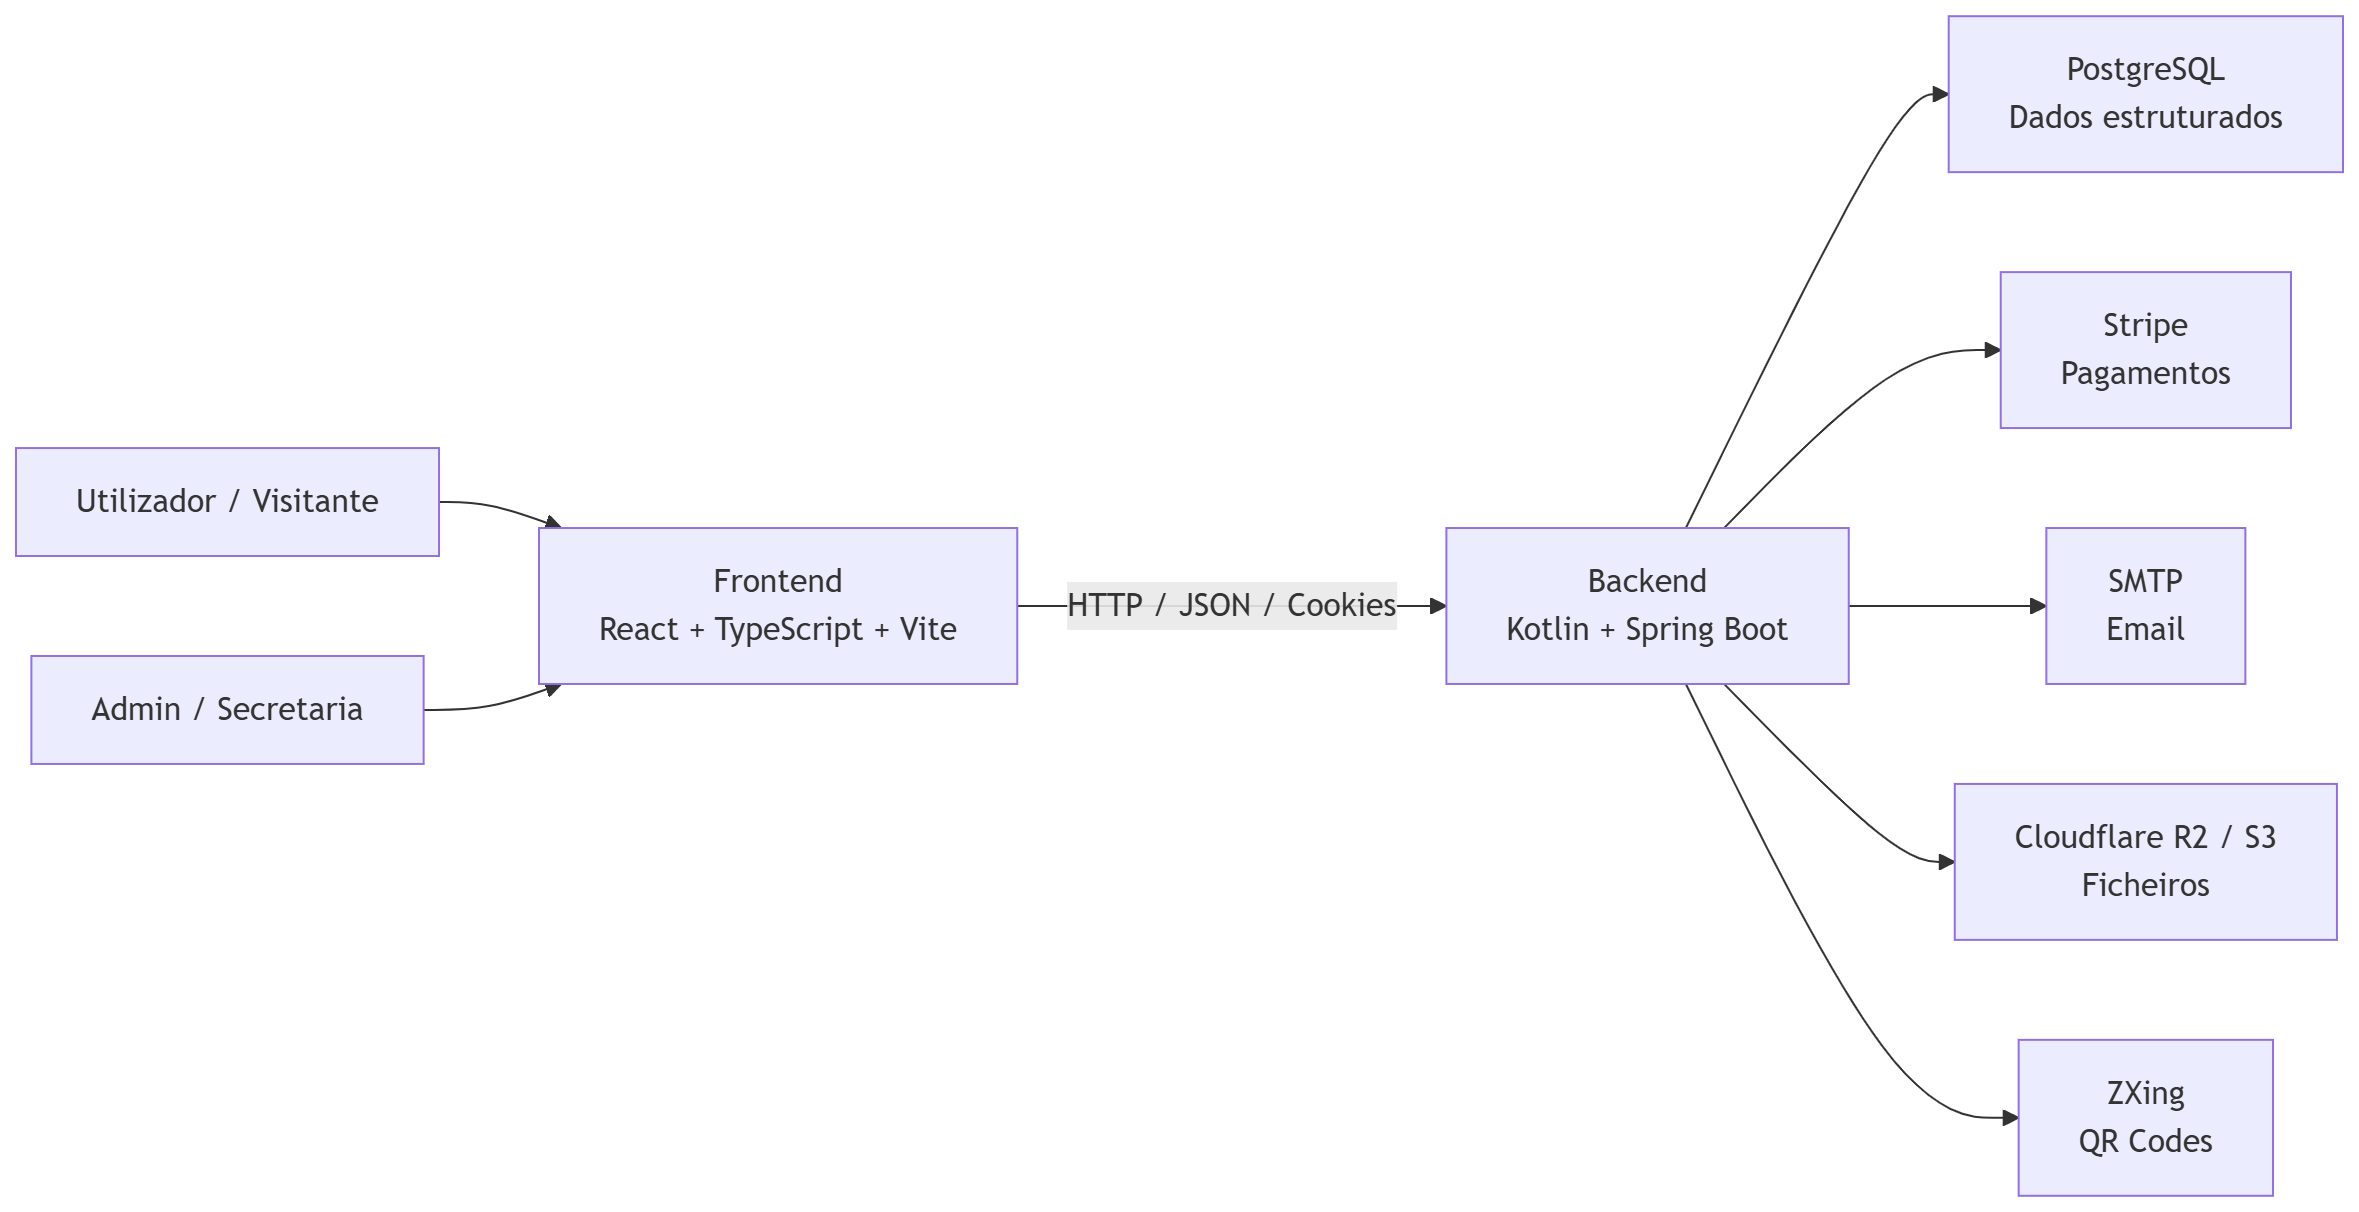
\includegraphics[width=\textwidth]{./figures/architecture-context.png}
    \caption{Arquitetura geral da aplicação}
    \label{fig:architecture-context}
\end{figure}

Esta divisão permite separar responsabilidades e reduzir o acoplamento entre
componentes. O \textit{frontend} não acede diretamente à base de dados, fazendo
todos os pedidos através da API. O \textit{backend}, por sua vez, concentra a
validação das regras de negócio e controla o acesso aos dados e integrações.

\section{Arquitetura Modular}

O projeto foi organizado como uma aplicação multi-módulo. Esta decisão foi
tomada para separar claramente as responsabilidades internas do sistema e
evitar que todas as classes ficassem concentradas num único módulo. Embora esta
separação seja mais visível no \textit{backend}, ela influencia a forma como a
aplicação é mantida e testada.

A organização em módulos permite:

\begin{itemize}
    \item isolar a lógica de domínio de detalhes tecnológicos;
    \item impedir que os controladores dependam diretamente da base de dados;
    \item substituir implementações de repositórios sem alterar os serviços;
    \item testar regras de negócio sem iniciar a aplicação completa;
    \item tornar explícitas as dependências entre camadas;
    \item facilitar a evolução futura do projeto.
\end{itemize}

Os principais módulos do \textit{backend} são:

\begin{itemize}
    \item \texttt{domain}: entidades, enumerações, validações e regras puras de
    domínio;
    \item \texttt{repository}: contratos de acesso a dados;
    \item \texttt{repository-jdbi}: implementação concreta dos repositórios em
    PostgreSQL através de JDBI;
    \item \texttt{services}: casos de uso e lógica de negócio da aplicação;
    \item \texttt{http}: controladores REST, modelos HTTP e pipeline de
    autenticação;
    \item \texttt{host}: módulo de arranque e configuração da aplicação Spring
    Boot.
\end{itemize}

\begin{figure}[H]
    \centering
    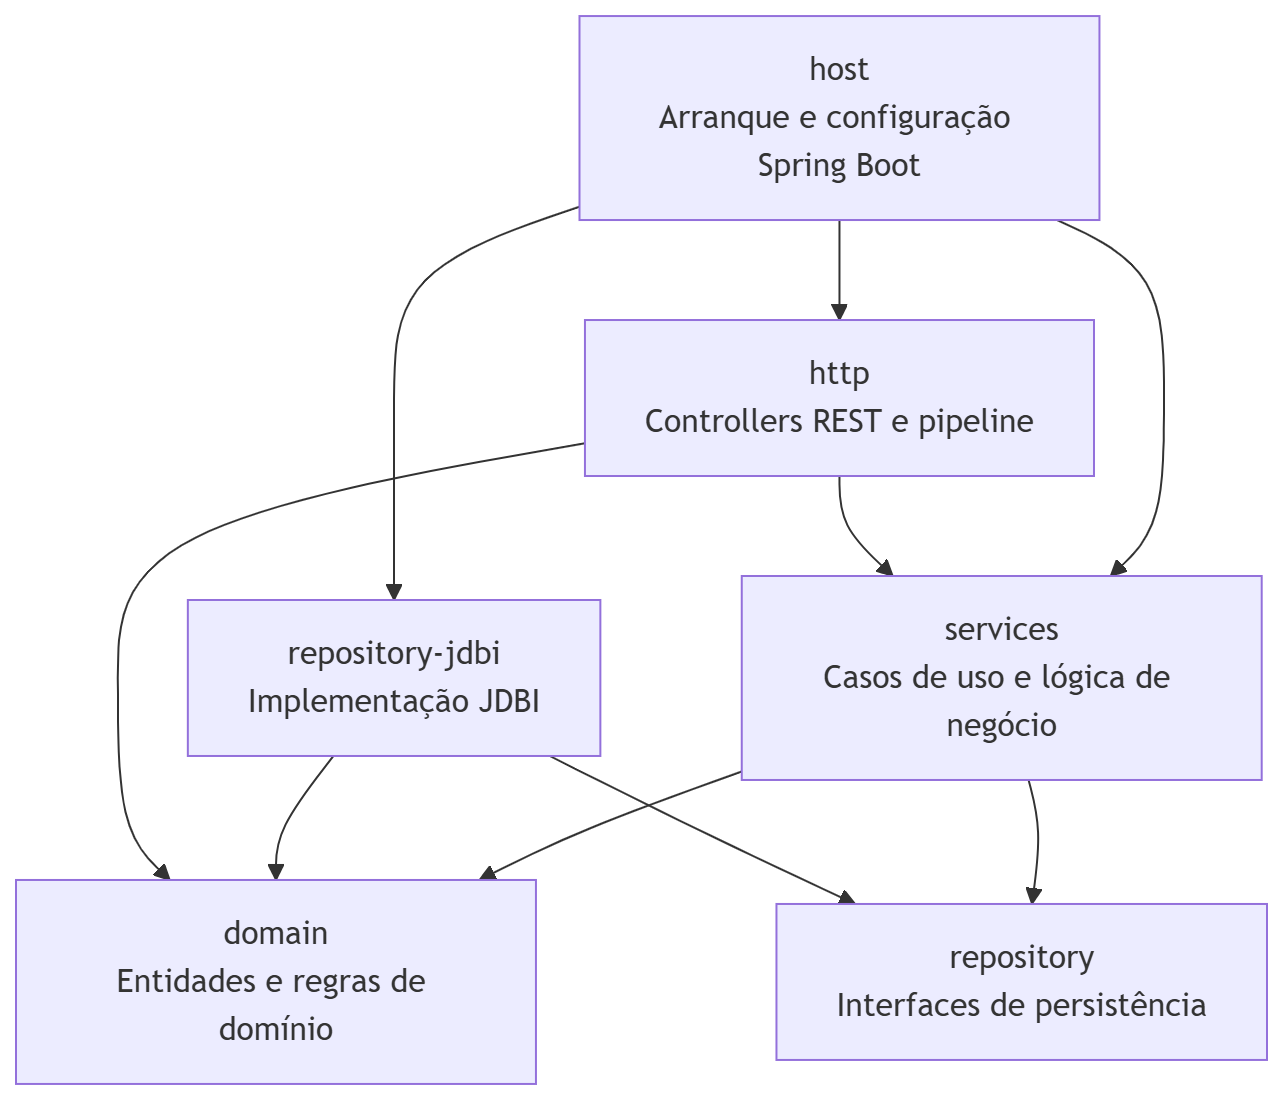
\includegraphics[width=\textwidth]{./figures/backend-modules.png}
    \caption{Dependências entre os módulos do backend}
    \label{fig:backend-modules}
\end{figure}

\section{Principais Fluxos da Aplicação}

Esta secção descreve os principais fluxos de utilização suportados pela
aplicação.

\subsection{Fluxo de Autenticação}

O fluxo de autenticação começa quando o utilizador submete as suas credenciais
no \textit{frontend}. O \textit{backend} valida a palavra-passe e, em caso de
sucesso, cria um \textit{token} de sessão. Esse \textit{token} é enviado ao
cliente através de um \textit{cookie} e usado nos pedidos seguintes.

\begin{figure}[H]
    \centering
    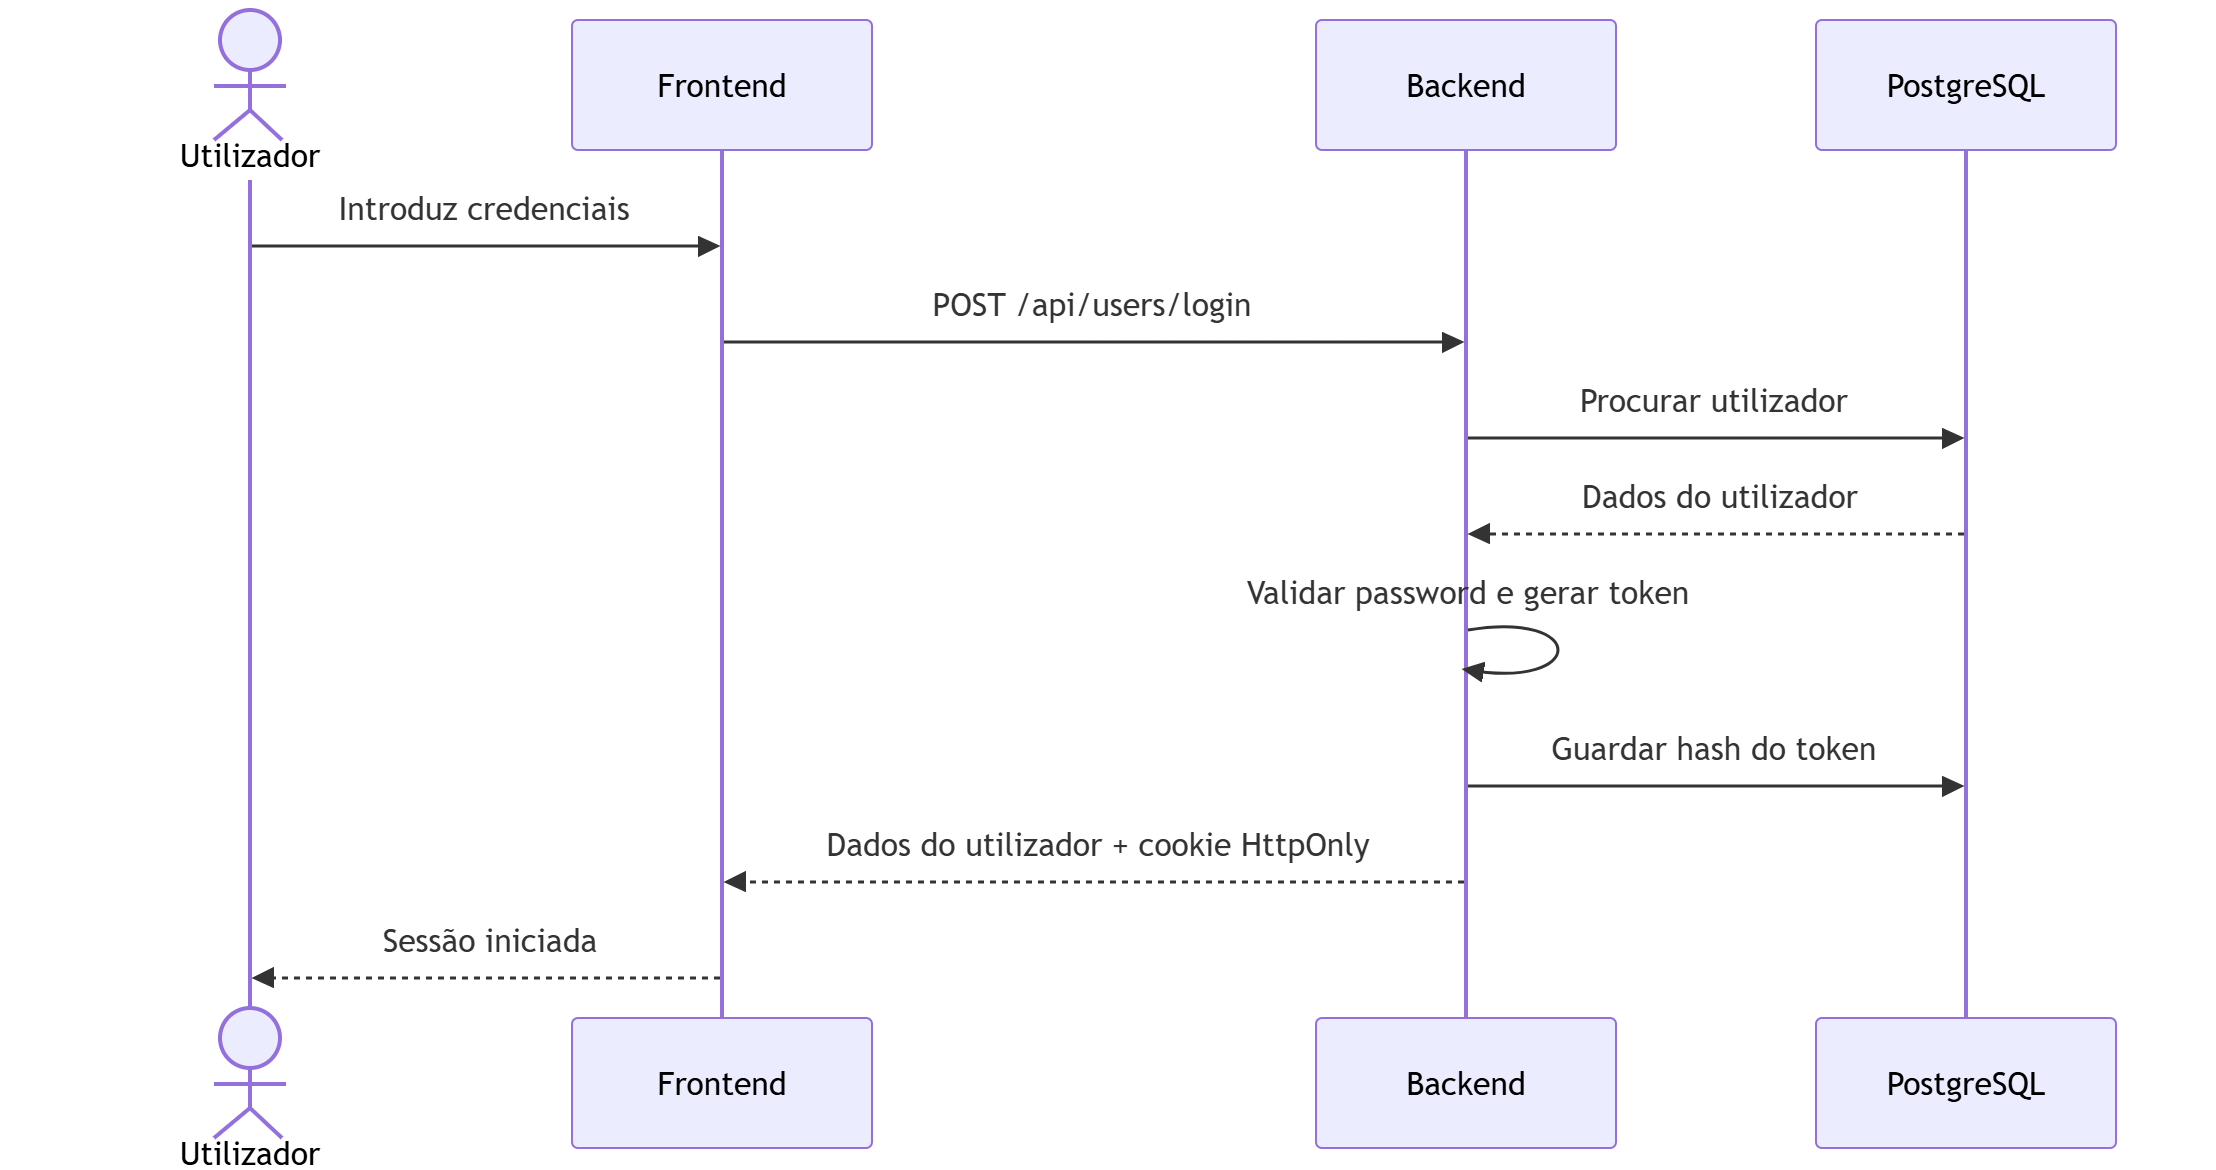
\includegraphics[width=0.9\textwidth]{./figures/auth-flow.png}
    \caption{Fluxo de autenticação}
    \label{fig:auth-flow}
\end{figure}

\subsection{Fluxo de Inscrição de Sócio}

A adesão de sócio é um dos fluxos centrais da aplicação. O utilizador preenche
um formulário no \textit{frontend}, que envia os dados para a API. O
\textit{backend} valida os dados, cria o registo de sócio em estado pendente e
disponibiliza-o para análise pela secretaria ou administração.

\begin{figure}[H]
    \centering
    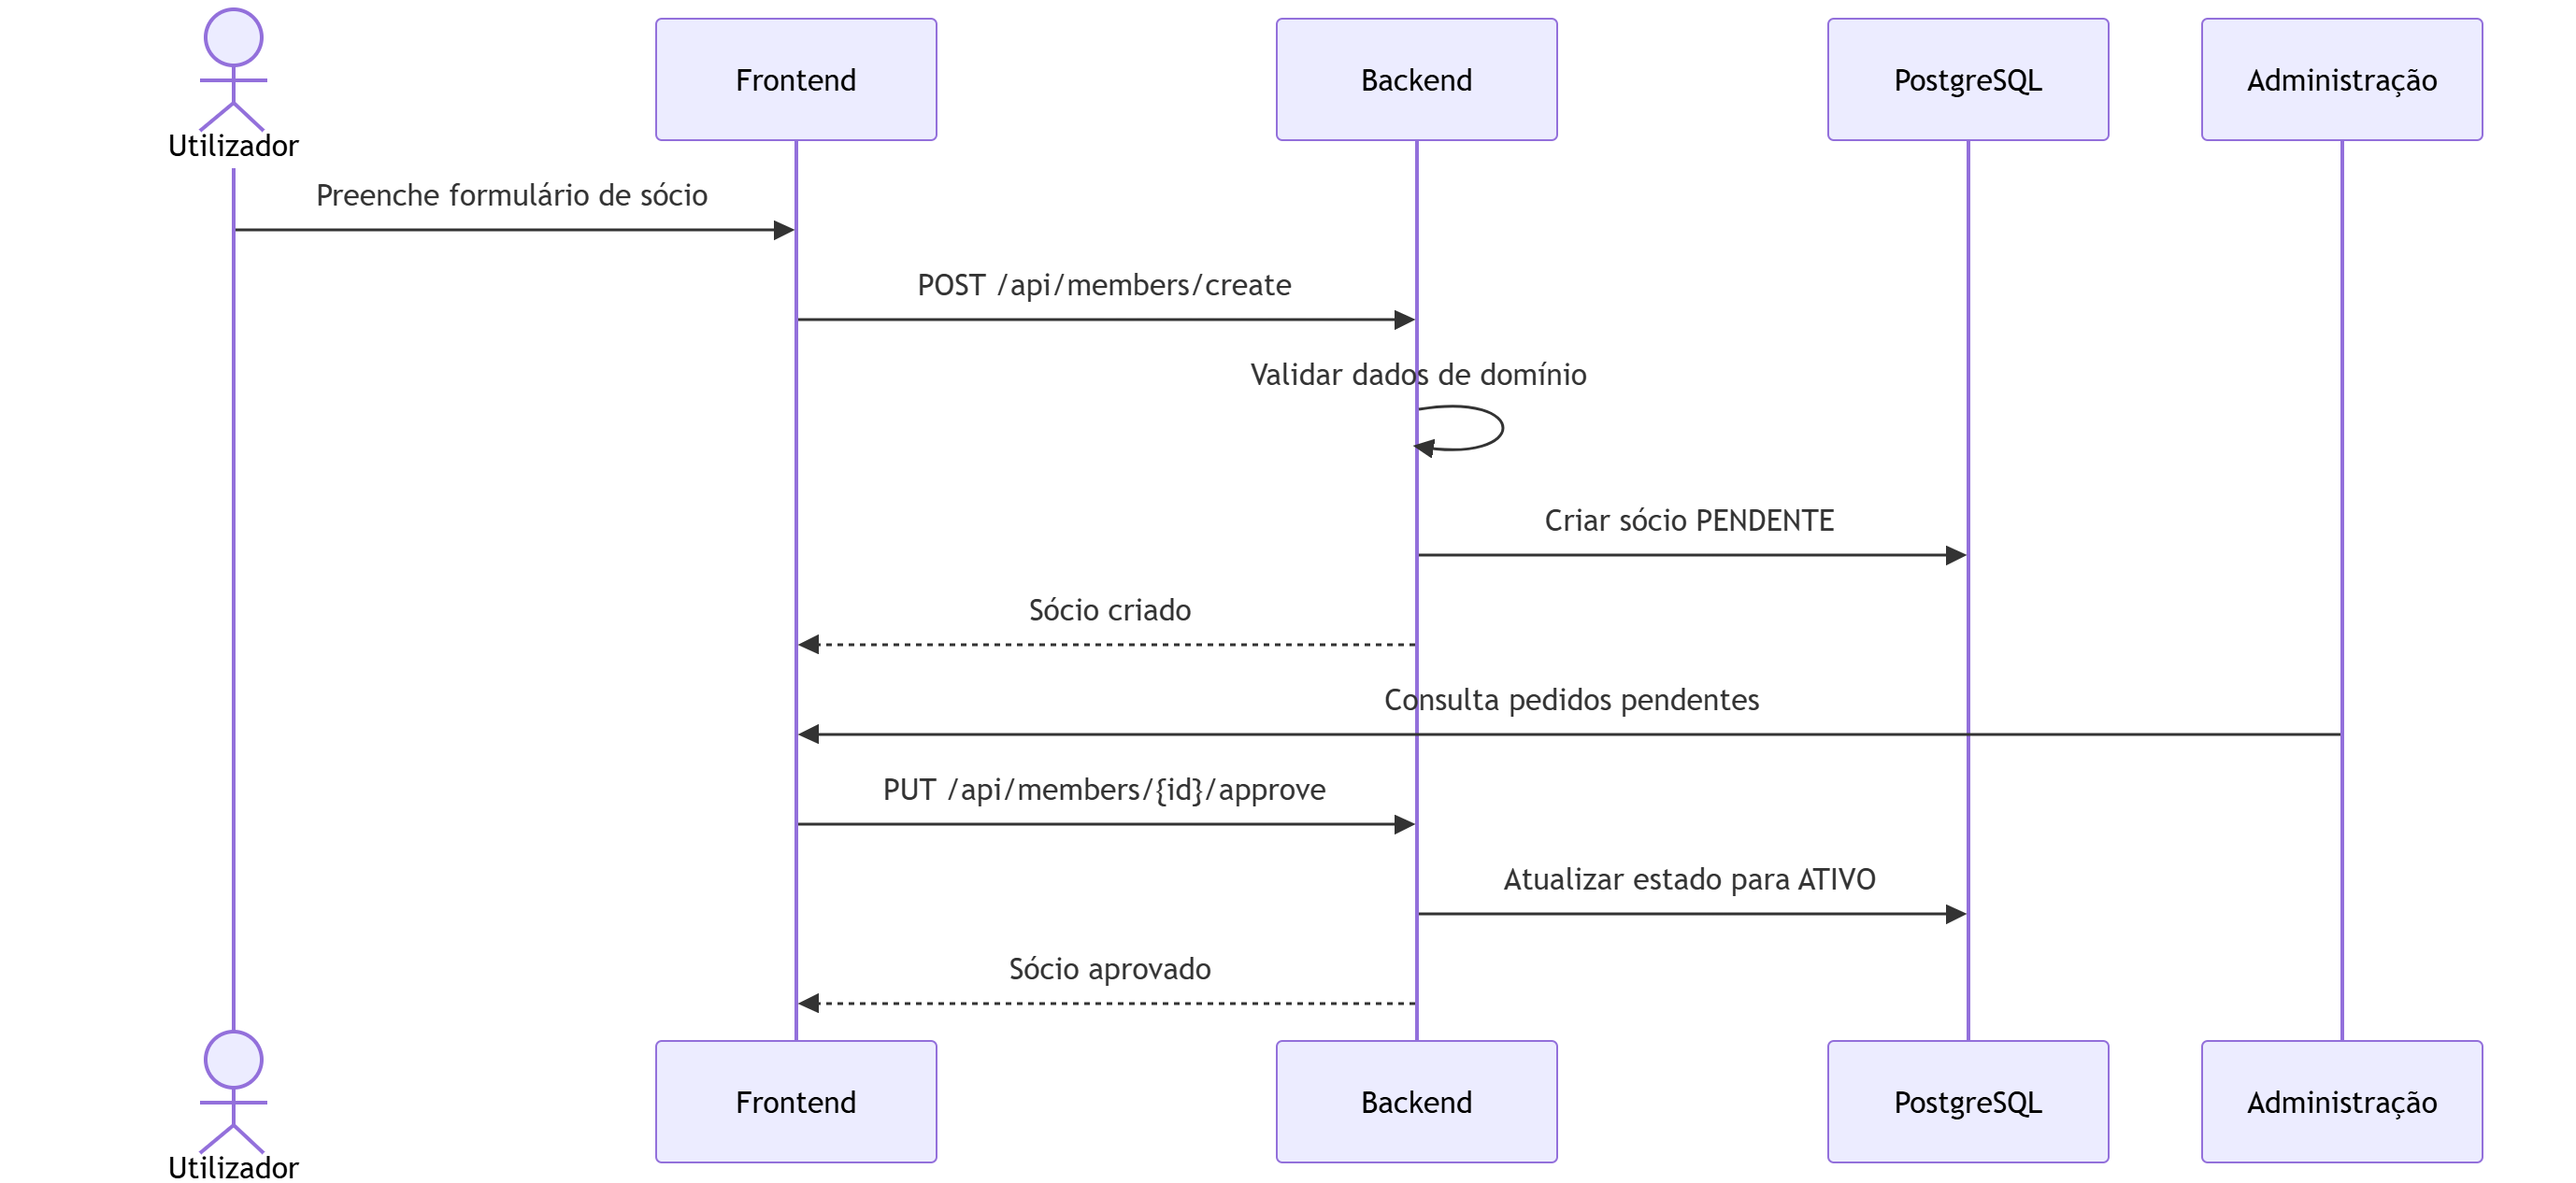
\includegraphics[width=0.9\textwidth]{./figures/member-registration-flow.png}
    \caption{Fluxo de adesão de sócio}
    \label{fig:member-registration-flow}
\end{figure}

\subsection{Fluxo de Inscrição de Atleta}

A inscrição de atleta é mais complexa, uma vez que envolve dados pessoais,
dados desportivos e encarregados de educação. No \textit{backend}, esta
operação cria, numa única transação, o sócio associado, o atleta e os
respetivos encarregados. Esta abordagem garante que não existem atletas
incompletos caso alguma parte da operação falhe.

\begin{figure}[H]
    \centering
    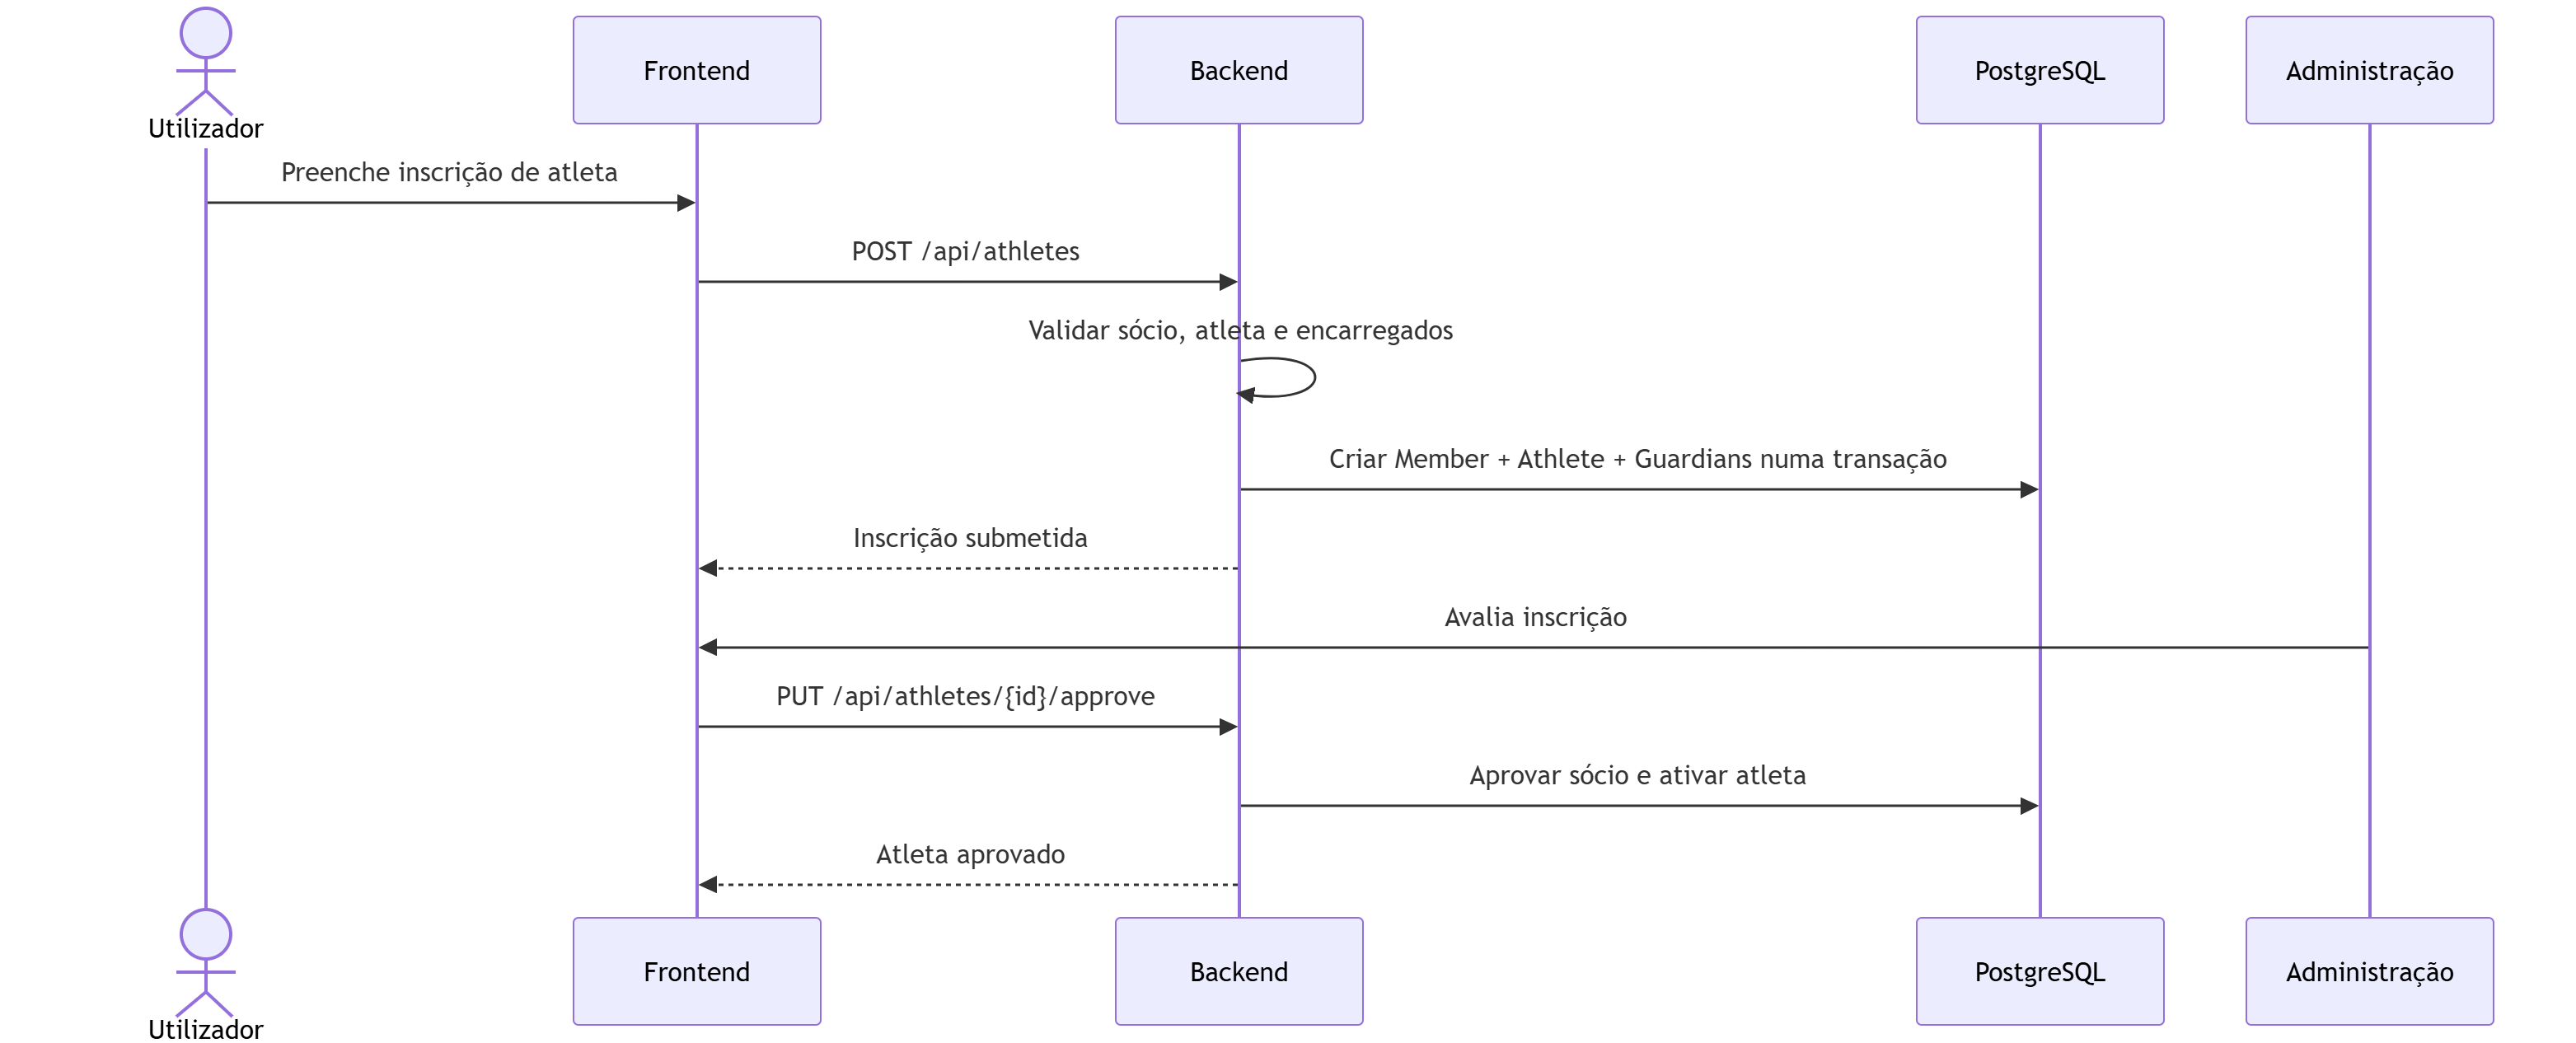
\includegraphics[width=0.9\textwidth]{./figures/athlete-registration-flow.png}
    \caption{Fluxo de inscrição de atleta}
    \label{fig:athlete-registration-flow}
\end{figure}

\subsection{Fluxo de Patrocínio}

No fluxo de patrocínio, o utilizador escolhe uma opção disponível, preenche os
dados do patrocinador e submete o pedido. A secretaria ou administração pode
posteriormente aprovar o pedido, marcar o pagamento e acompanhar o estado do
contrato.

\begin{figure}[H]
    \centering
    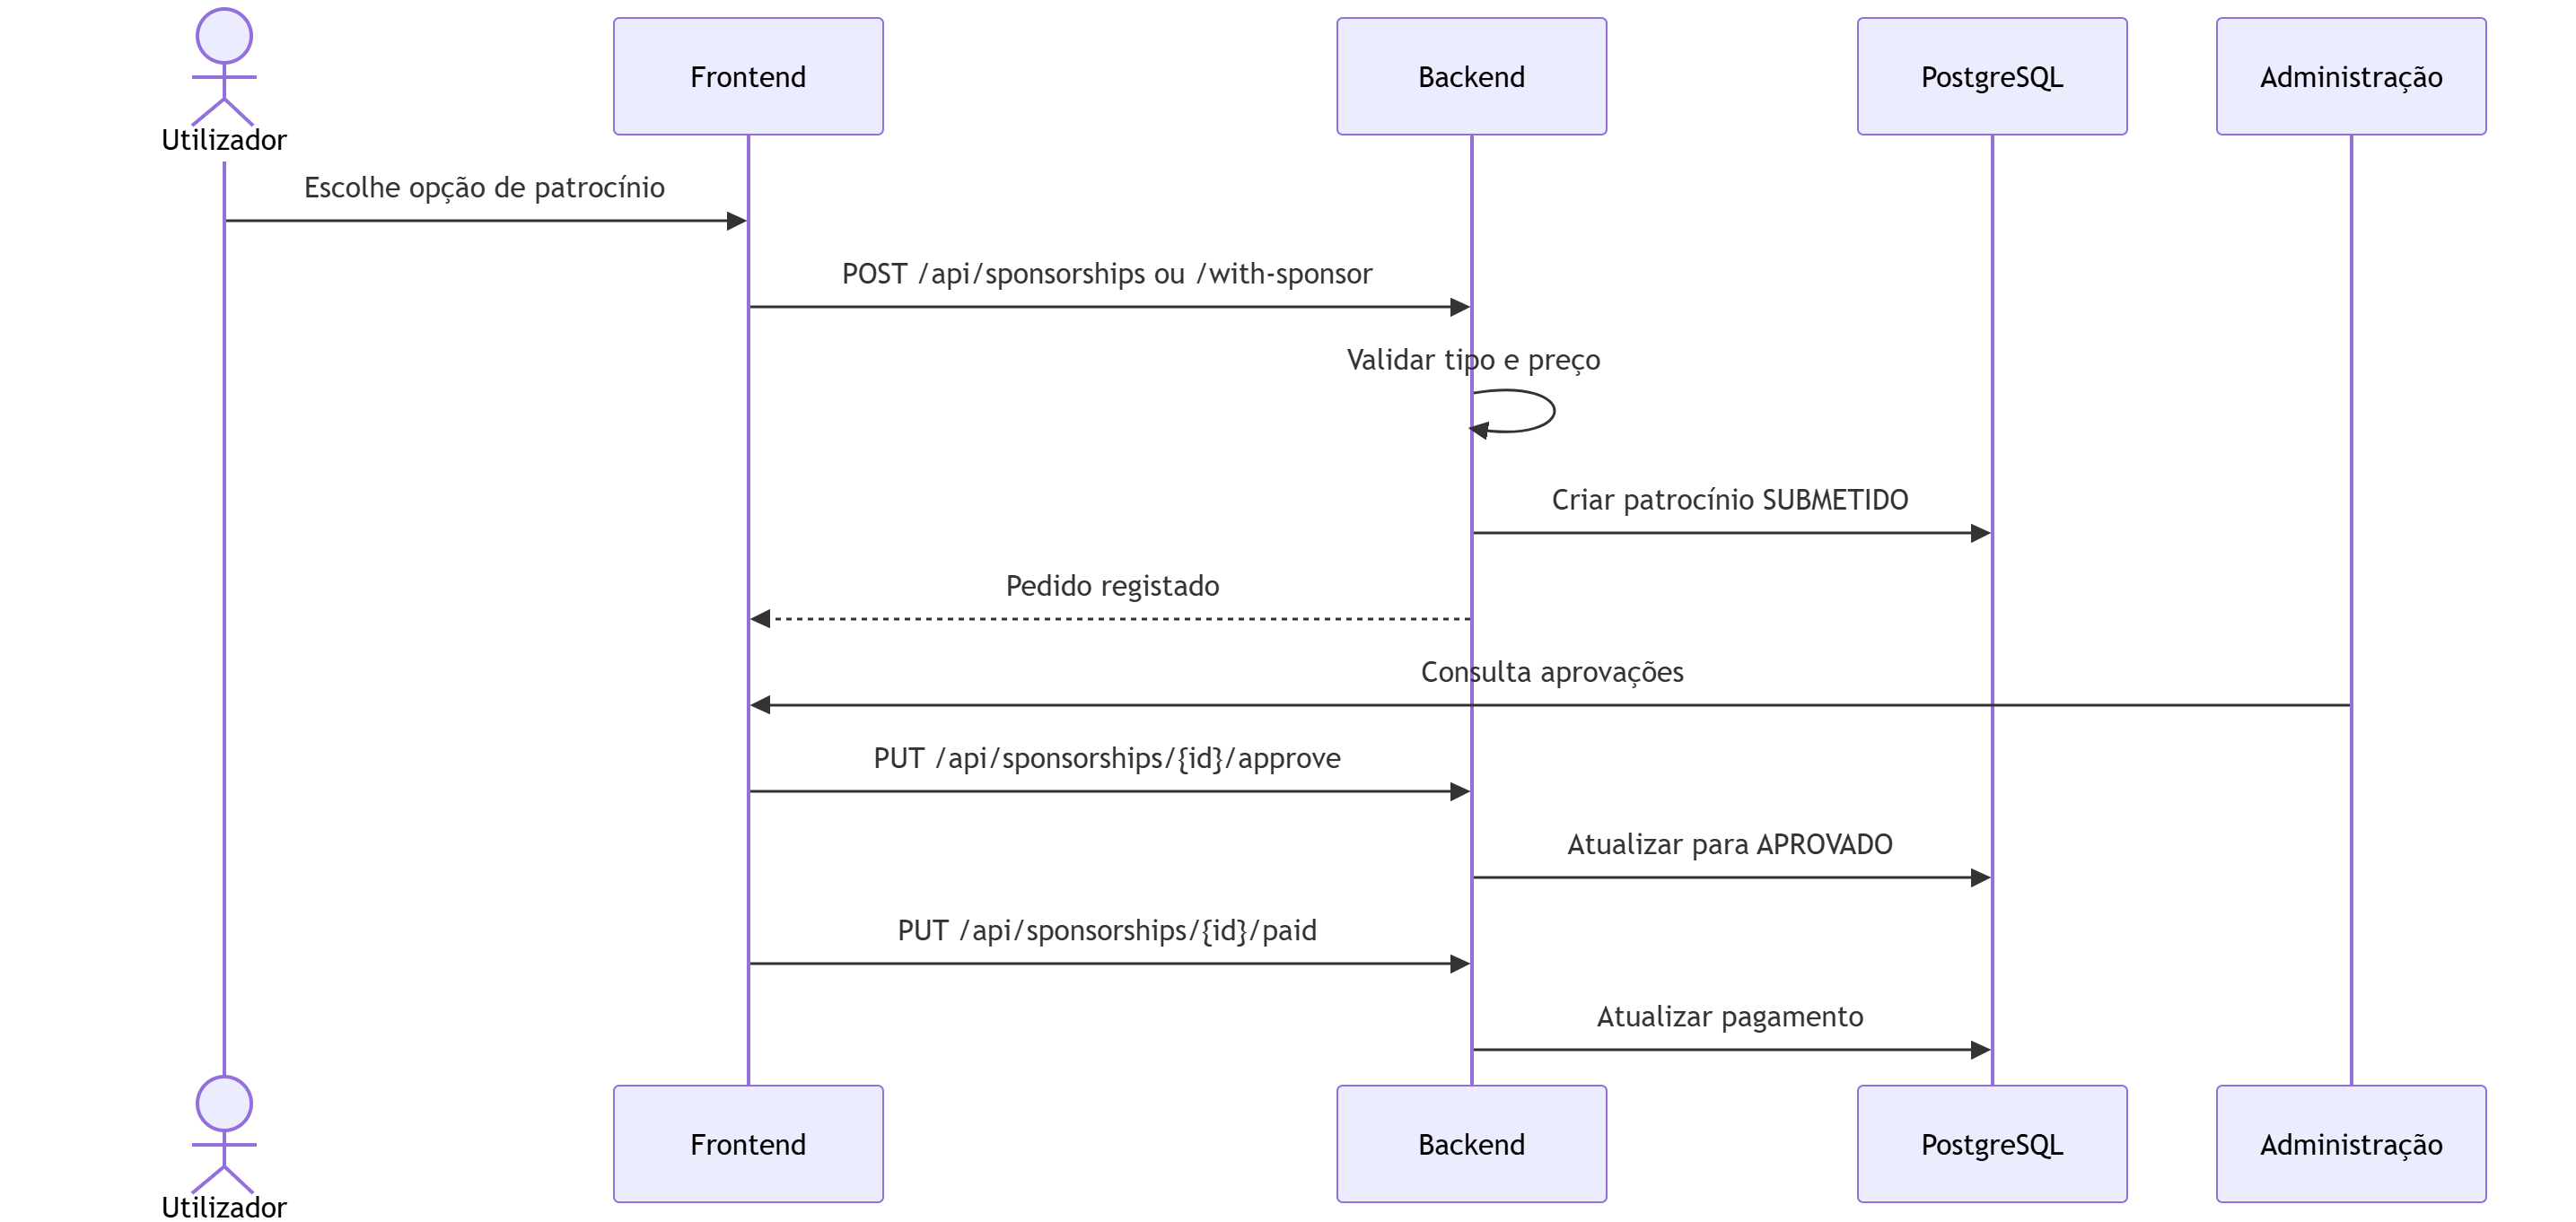
\includegraphics[width=0.9\textwidth]{./figures/sponsorship-flow.png}
    \caption{Fluxo de submissão e aprovação de patrocínio}
    \label{fig:sponsorship-flow}
\end{figure}

\subsection{Fluxo de Compra de Bilhetes}

Na compra de bilhetes, o utilizador seleciona um evento e o setor pretendido.
Quando o bilhete é de sócio, a aplicação valida o número de sócio e a data de
nascimento. Depois é criada uma sessão de pagamento na Stripe. Quando o
pagamento é confirmado, o \textit{backend} confirma os bilhetes, gera os
códigos QR e envia a confirmação por email.

\begin{figure}[H]
    \centering
    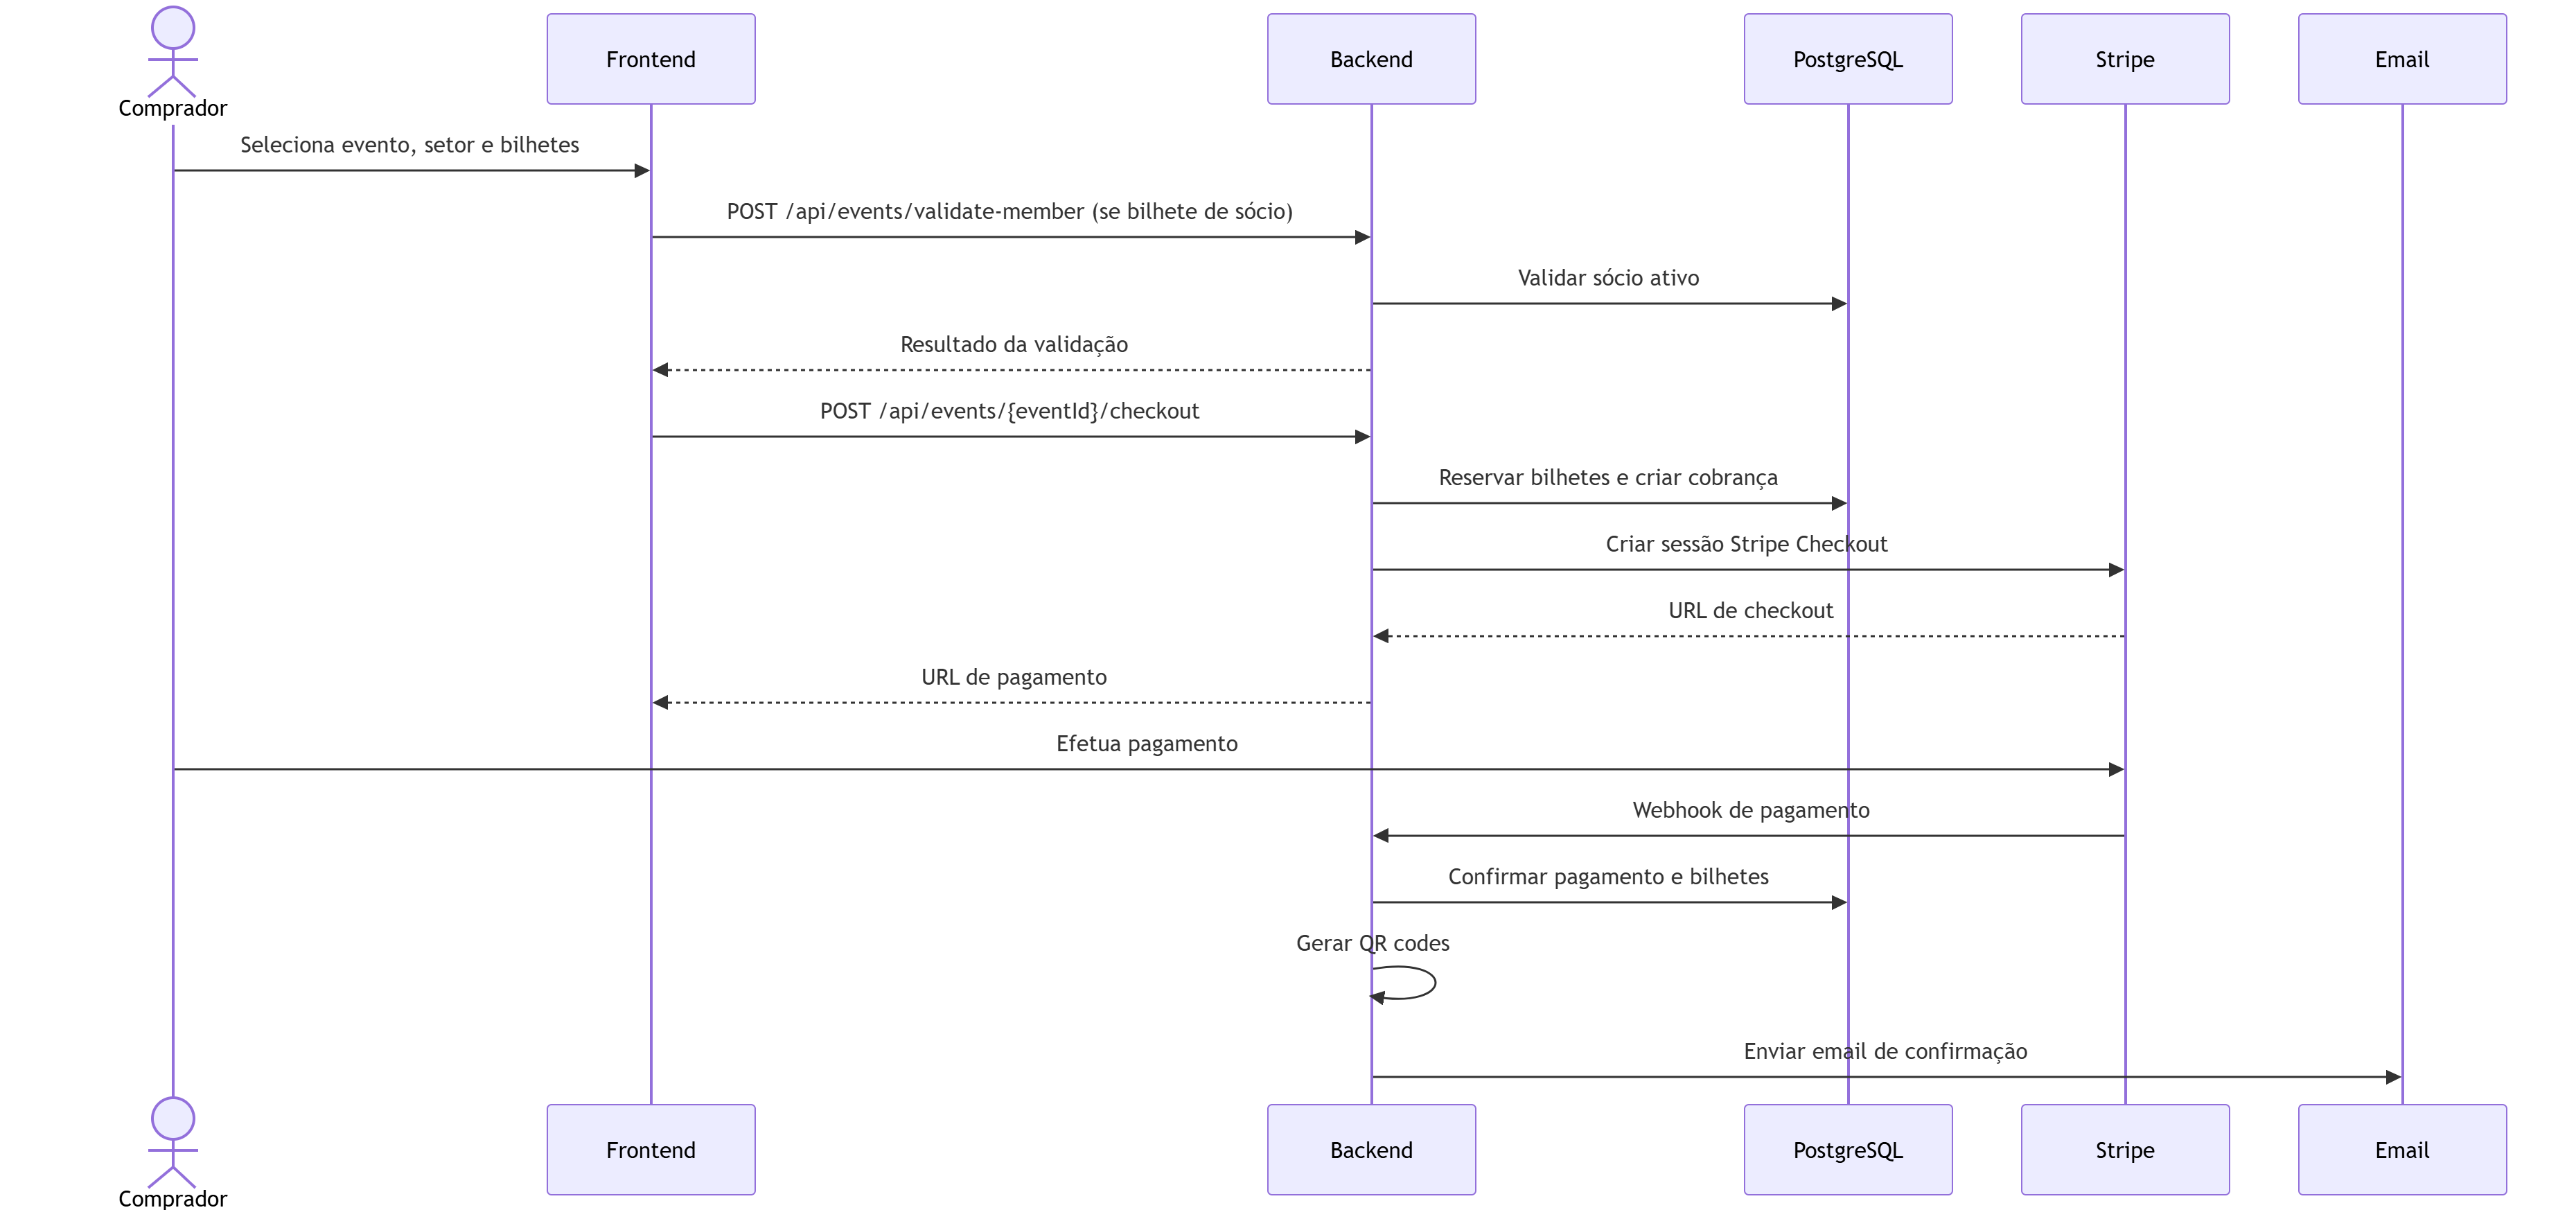
\includegraphics[width=\textwidth]{./figures/ticket-payment-flow.png}
    \caption{Fluxo de compra de bilhetes e confirmação de pagamento}
    \label{fig:ticket-payment-flow}
\end{figure}

\section{Síntese}

A JagozApp foi desenhada para responder a um conjunto alargado de necessidades
de gestão de um clube desportivo local. A separação entre \textit{frontend},
\textit{backend}, base de dados e integrações externas permite organizar o
sistema de forma clara. A adoção de uma arquitetura multi-módulo no
\textit{backend} reforça esta separação, promovendo manutenção, testabilidade
e evolução futura.

Os requisitos definidos cobrem os processos essenciais do clube, desde a gestão
de sócios e atletas até à bilhética, pagamentos, patrocínios e documentos. Os
diagramas apresentados ajudam a compreender como estes processos atravessam as
várias camadas da aplicação e como cada componente contribui para o
funcionamento global do sistema.


% Capitulo 4
\chapter{Backend}

Este capítulo está organizado em seis secções. A primeira é dedicada à 
estrutura geral da aplicação; a segunda foca-se nos repositórios e no modelo 
de dados; a terceira é referente aos serviços; a quarta trata dos 
controladores; a quinta é focada no processo de autenticação e autorização; 
e por fim, a sexta secção descreve as integrações com serviços externos.

O backend da aplicação JagozApp fornece uma interface de comunicação entre o 
\textit{frontend} e a lógica central da aplicação através de uma Web API. Uma 
Web API (\textit{Application Programming Interface}) é, no fundo, um conjunto 
de \textit{endpoints} expostos sobre o protocolo HTTP (\textit{Hypertext 
Transfer Protocol}), que permite a diferentes aplicações comunicarem entre 
si.

O backend foi implementado na linguagem Kotlin~\cite{kotlin}, utilizando a 
framework Spring Boot~\cite{springboot}, que oferece um conjunto de abstrações 
e configurações que aceleram o desenvolvimento e promovem boas práticas. Esta 
framework permite a construção de APIs REST de forma estruturada e eficiente. 
Uma das principais vantagens do Spring é o suporte nativo a conceitos 
fundamentais como:

\begin{itemize}
    \item Inversão de controlo (IoC): permite delegar à framework a 
    responsabilidade de instanciar e gerir o ciclo de vida de objetos, 
    facilitando o desacoplamento entre componentes;
    \item Injeção de dependências (DI): injeta automaticamente as dependências 
    necessárias nos componentes da aplicação;
    \item Separação de responsabilidades: através da arquitetura em camadas 
    (\textit{controllers}, \textit{services}, \textit{repositories}), incentiva 
    a modularidade e organização do código.
\end{itemize}

\section{Estrutura}

O backend da aplicação foi desenvolvido segundo uma arquitetura modular e 
orientada a serviços, com uma clara separação de responsabilidades entre as 
diferentes camadas. Esta abordagem facilita a manutenção, a organização, a realização de testes e a 
extensibilidade do sistema.

A organização do código está dividida em vários módulos, cada um com uma 
responsabilidade bem definida:

\begin{itemize}
    \item \texttt{domain}: contém as entidades, enumerações e a lógica de 
    domínio, independente de qualquer tecnologia externa;
    \item \texttt{services}: contém a lógica de negócio da aplicação, 
    organizada em casos de uso;
    \item \texttt{repository}: define as interfaces de acesso a dados, sem 
    qualquer dependência da tecnologia de persistência utilizada;
    \item \texttt{repository-jdbi}: contém a implementação concreta das 
    interfaces de repositório, recorrendo à biblioteca JDBI;
    \item \texttt{http}: contém os controladores REST e o respetivo 
    \textit{pipeline} de processamento de pedidos;
    \item \texttt{host}: módulo de arranque da aplicação Spring Boot, 
    responsável pela configuração e pela ligação entre todos os módulos.
\end{itemize}

A arquitetura segue o padrão comum de três camadas: controladores, serviços e 
repositórios. Adicionalmente, são utilizadas interfaces para abstrair o acesso 
a dados, o que permite alternar facilmente entre diferentes implementações 
(por exemplo, uma implementação em memória para testes e uma implementação 
JDBI para produção).

A seguir são descritos os principais componentes:

\begin{itemize}
    \item \textit{Controllers} ou controladores: são responsáveis por receber 
    e tratar os pedidos HTTP provenientes do \textit{frontend}. Traduzem os 
    pedidos da camada de apresentação para chamadas aos serviços da aplicação 
    e retornam as respostas apropriadas;
    \item \textit{Services} ou serviços: contêm a lógica de negócio da 
    aplicação. São responsáveis por coordenar as ações necessárias à execução 
    de cada operação;
    \item \textit{Repositories} ou repositórios: abstraem o acesso aos dados 
    persistentes. O acesso a dados estruturados é feito através da base de 
    dados relacional, enquanto o armazenamento de ficheiros é delegado a um 
    serviço de armazenamento dedicado.
\end{itemize}

Importa ainda destacar duas abstrações transversais a toda a aplicação. A 
primeira é o tipo \texttt{Either<L, R>}, que encapsula o sucesso 
(\texttt{Right}) ou a falha (\texttt{Left}) de uma operação. Os serviços 
seguem esta abordagem de retorno funcional, o que torna o tratamento de erros 
explícito e evita o recurso a exceções não controladas. A segunda é o 
\texttt{TransactionManager}, que permite que cada operação de um serviço seja 
executada no contexto de uma transação, garantindo a consistência das 
operações que envolvem múltiplos repositórios.


\section{Repositórios e Base de Dados}

Neste projeto, verificou-se a necessidade de uma divisão em dois tipos  de repositórios, cada um associado a uma forma de armazenamento distinta:

\begin{itemize}
    \item Repositório de dados -- responsável por armazenar e consultar dados 
    estruturados, como utilizadores, sócios, atletas, patrocínios, pagamentos 
    e eventos, através de uma base de dados relacional;
    \item Repositório de ficheiros -- responsável por armazenar os ficheiros 
    associados às entidades, como fotografias e documentos, através de um 
    serviço de armazenamento externo.
\end{itemize}

Ambos os repositórios são abstraídos através de interfaces, o que permite a substituição ou simulação de comportamentos para testes. As interfaces estão definidas no módulo \texttt{repository}, enquanto a sua implementação concreta 
reside no módulo \texttt{repository-jdbi}. Desta forma, as camadas de serviços e de controladores nunca dependem diretamente da tecnologia de persistência 
utilizada.

\subsection{Repositório de Dados}

Este repositório utiliza a base de dados relacional PostgreSQL~\cite{postgresql}, 
escolhida pelas seguintes razões:

\begin{itemize}
    \item Familiaridade;
    \item Documentação extensiva;
    \item Desempenho estável e fiável para dados relacionais;
    \item Facilidade de integração com bibliotecas Kotlin como o JDBI.
\end{itemize}

O acesso à base de dados é feito através da biblioteca JDBI~\cite{jdbi}, que 
permite executar \textit{queries} parametrizadas em SQL nativo com uma boa 
integração em Kotlin, mantendo o controlo explícito sobre as operações 
realizadas. Ao contrário de soluções baseadas em ORM (Object-Relational Mapping), esta abordagem evita 
camadas de abstração adicionais e mantém o SQL visível e sob controlo do 
programador.

\subsubsection*{Base de dados}

O modelo de dados está organizado em torno de várias áreas funcionais da 
aplicação. As principais entidades são descritas a seguir.

A entidade \texttt{User} representa um utilizador da aplicação e armazena o 
identificador, o \textit{email}, o nome de utilizador, a informação de 
validação da palavra-passe e o papel (\texttt{role}) atribuído. Cada 
utilizador pode estar opcionalmente associado a um sócio ativo. A informação 
de autenticação é complementada pela entidade \texttt{Token}, que representa 
as sessões ativas de cada utilizador.

A entidade \texttt{Member} corresponde a um sócio do clube e concentra os seus 
dados pessoais e administrativos, como o número de sócio, o nome completo, a 
data de nascimento, os contactos, a morada, o NIF, a categoria, o estado e a 
quota associada. A entidade \texttt{Athlete} representa um atleta e está sempre 
associada a um sócio, numa relação de um para um. Um atleta contém informação 
desportiva e escolar, bem como uma lista de encarregados de educação, 
representados pela entidade \texttt{Guardian}.

A organização das equipas é feita através das entidades \texttt{TeamGroup} 
(grupo ou modalidade) e \texttt{TeamCategory} (escalão), às quais os atletas 
são associados. A estas juntam-se entidades dedicadas à definição das tabelas 
de preços.

A área de patrocínios é composta pela entidade \texttt{Sponsor}, que representa 
um patrocinador, e pela entidade \texttt{Sponsorship}, que representa um 
contrato de patrocínio. Existem ainda entidades de catálogo que definem as 
opções de patrocínio disponíveis.

A componente financeira assenta nas entidades \texttt{Charge} (cobrança), 
\texttt{ChargeItem} (item de uma cobrança) e \texttt{Payment} (pagamento). Uma 
cobrança pode estar associada a um sócio ou a um contrato de patrocínio, e dá 
origem a um ou mais pagamentos.

Por fim, a área de eventos é composta pela entidade \texttt{Event} (jogo), pela 
entidade \texttt{EventSector} (setor com lotação) e pela entidade 
\texttt{Ticket} (bilhete), que suporta a funcionalidade relacionada com os bilhetes.

Vários campos, como o papel de um utilizador, o estado de um sócio ou o estado 
de um contrato de patrocínio, são restritos a um conjunto de valores 
predefinidos, implementados como enumerações para garantir a consistência e a 
integridade dos dados.

Dado o número de entidades envolvidas, o modelo de dados é apresentado em 
quatro diagramas, organizados por área funcional. A 
Figura~\ref{fig:er-nucleo} representa o núcleo de utilizadores, sócios e 
atletas; a Figura~\ref{fig:er-equipas} representa a organização das equipas e 
as tabelas de preços; a Figura~\ref{fig:er-patrocinios} representa a área de 
patrocínios; e a Figura~\ref{fig:er-financas-eventos} representa as áreas 
financeira e de eventos. As enumerações associadas a cada área estão 
representadas no respetivo diagrama.

\begin{figure}[H]
    \centering
    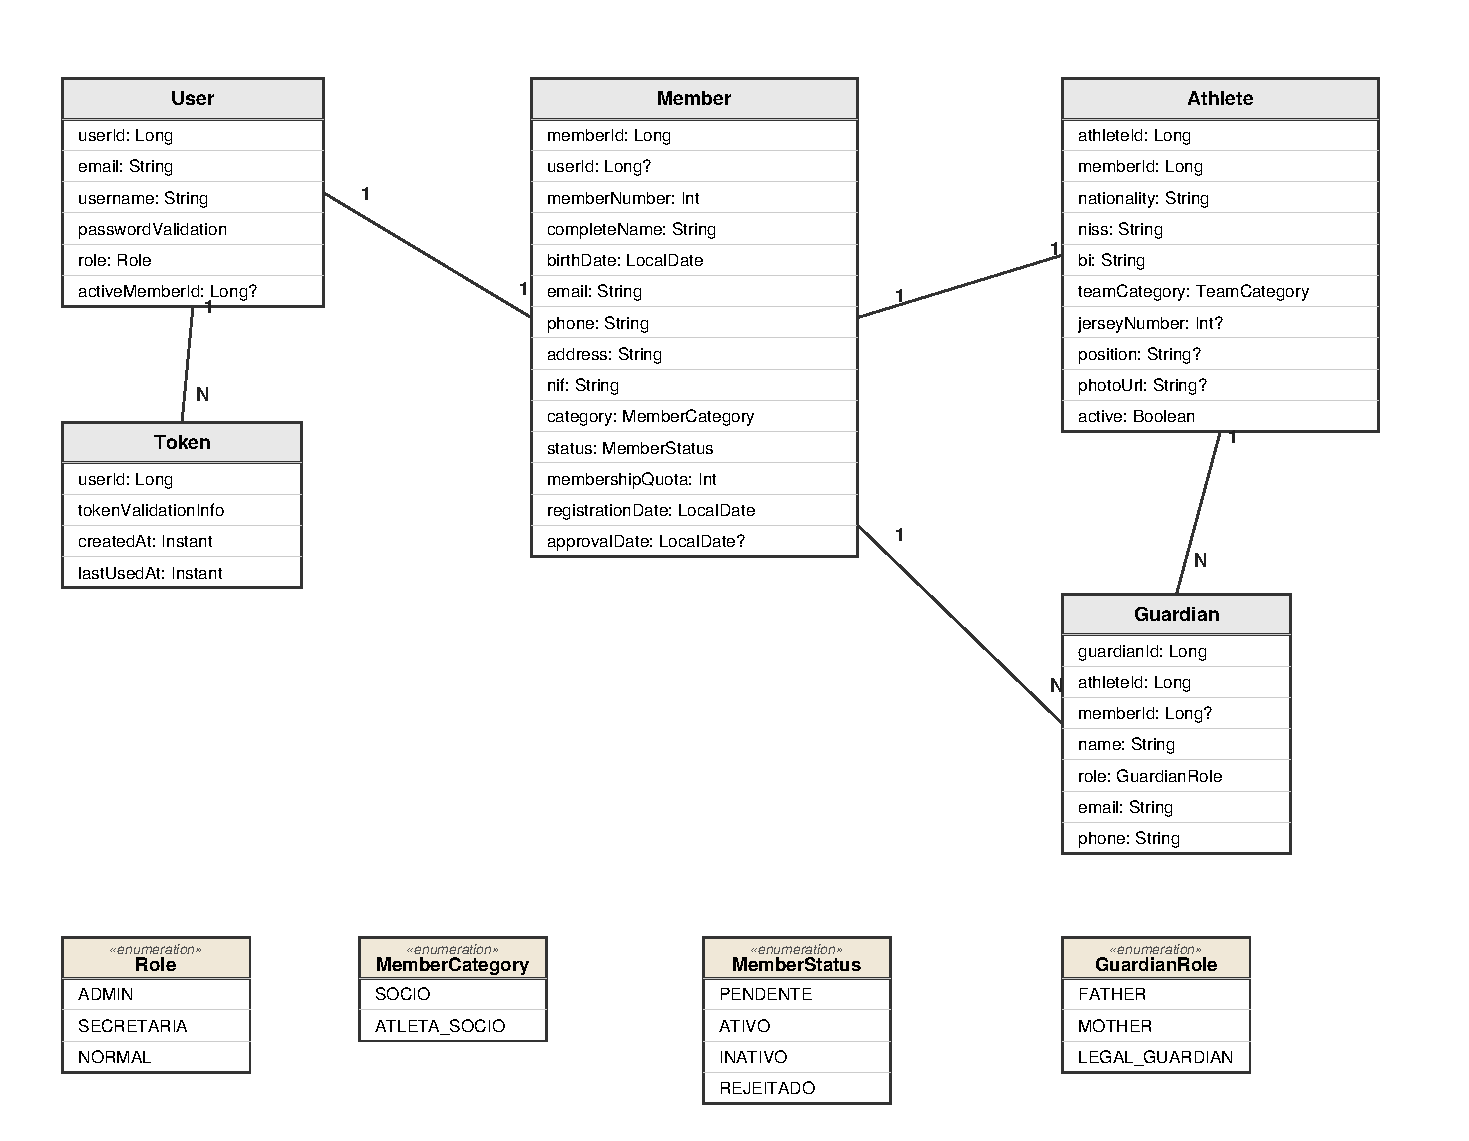
\includegraphics[width=\textwidth]{./figures/er-nucleo.pdf}
    \caption{Modelo de dados -- utilizadores, sócios e atletas}
    \label{fig:er-nucleo}
\end{figure}

\begin{figure}[H]
    \centering
    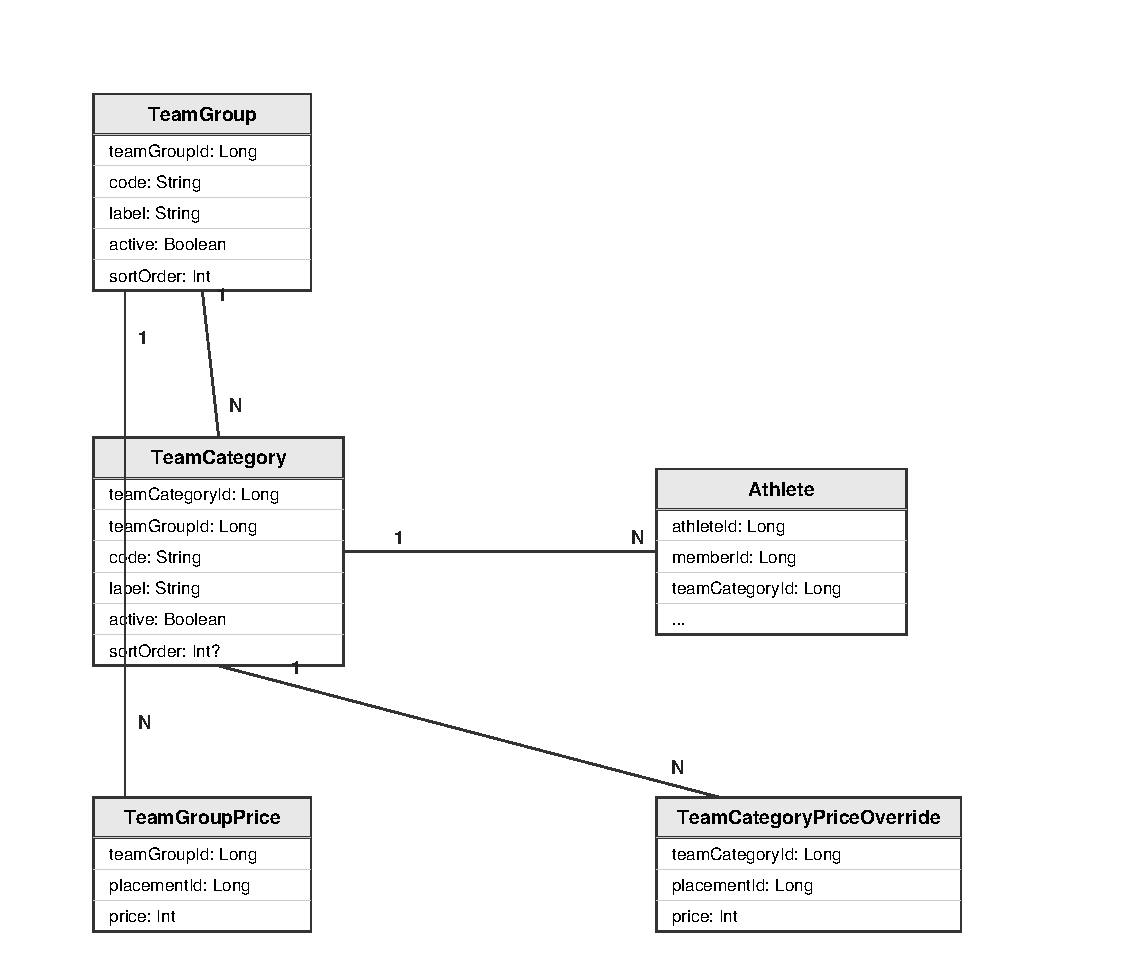
\includegraphics[width=0.75\textwidth]{./figures/er-equipas.pdf}
    \caption{Modelo de dados -- equipas e tabelas de preços}
    \label{fig:er-equipas}
\end{figure}

\begin{figure}[H]
    \centering
    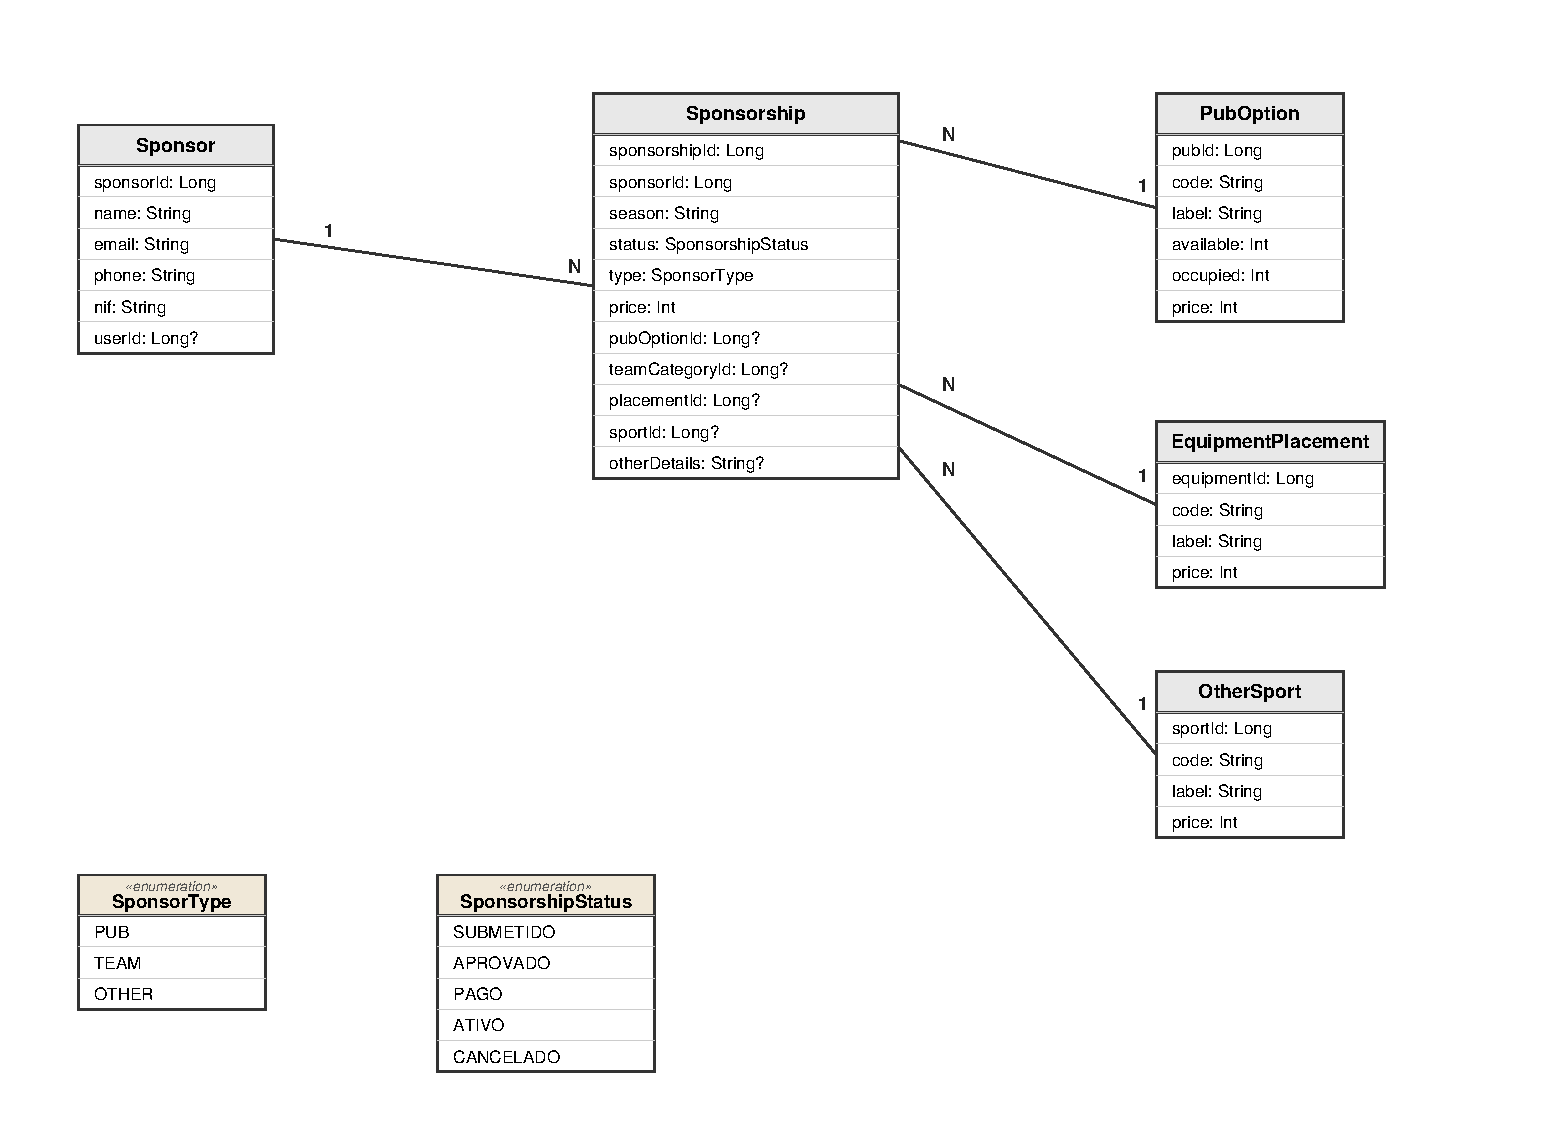
\includegraphics[width=\textwidth]{./figures/er-patrocinios.pdf}
    \caption{Modelo de dados -- patrocínios}
    \label{fig:er-patrocinios}
\end{figure}

\begin{figure}[H]
    \centering
    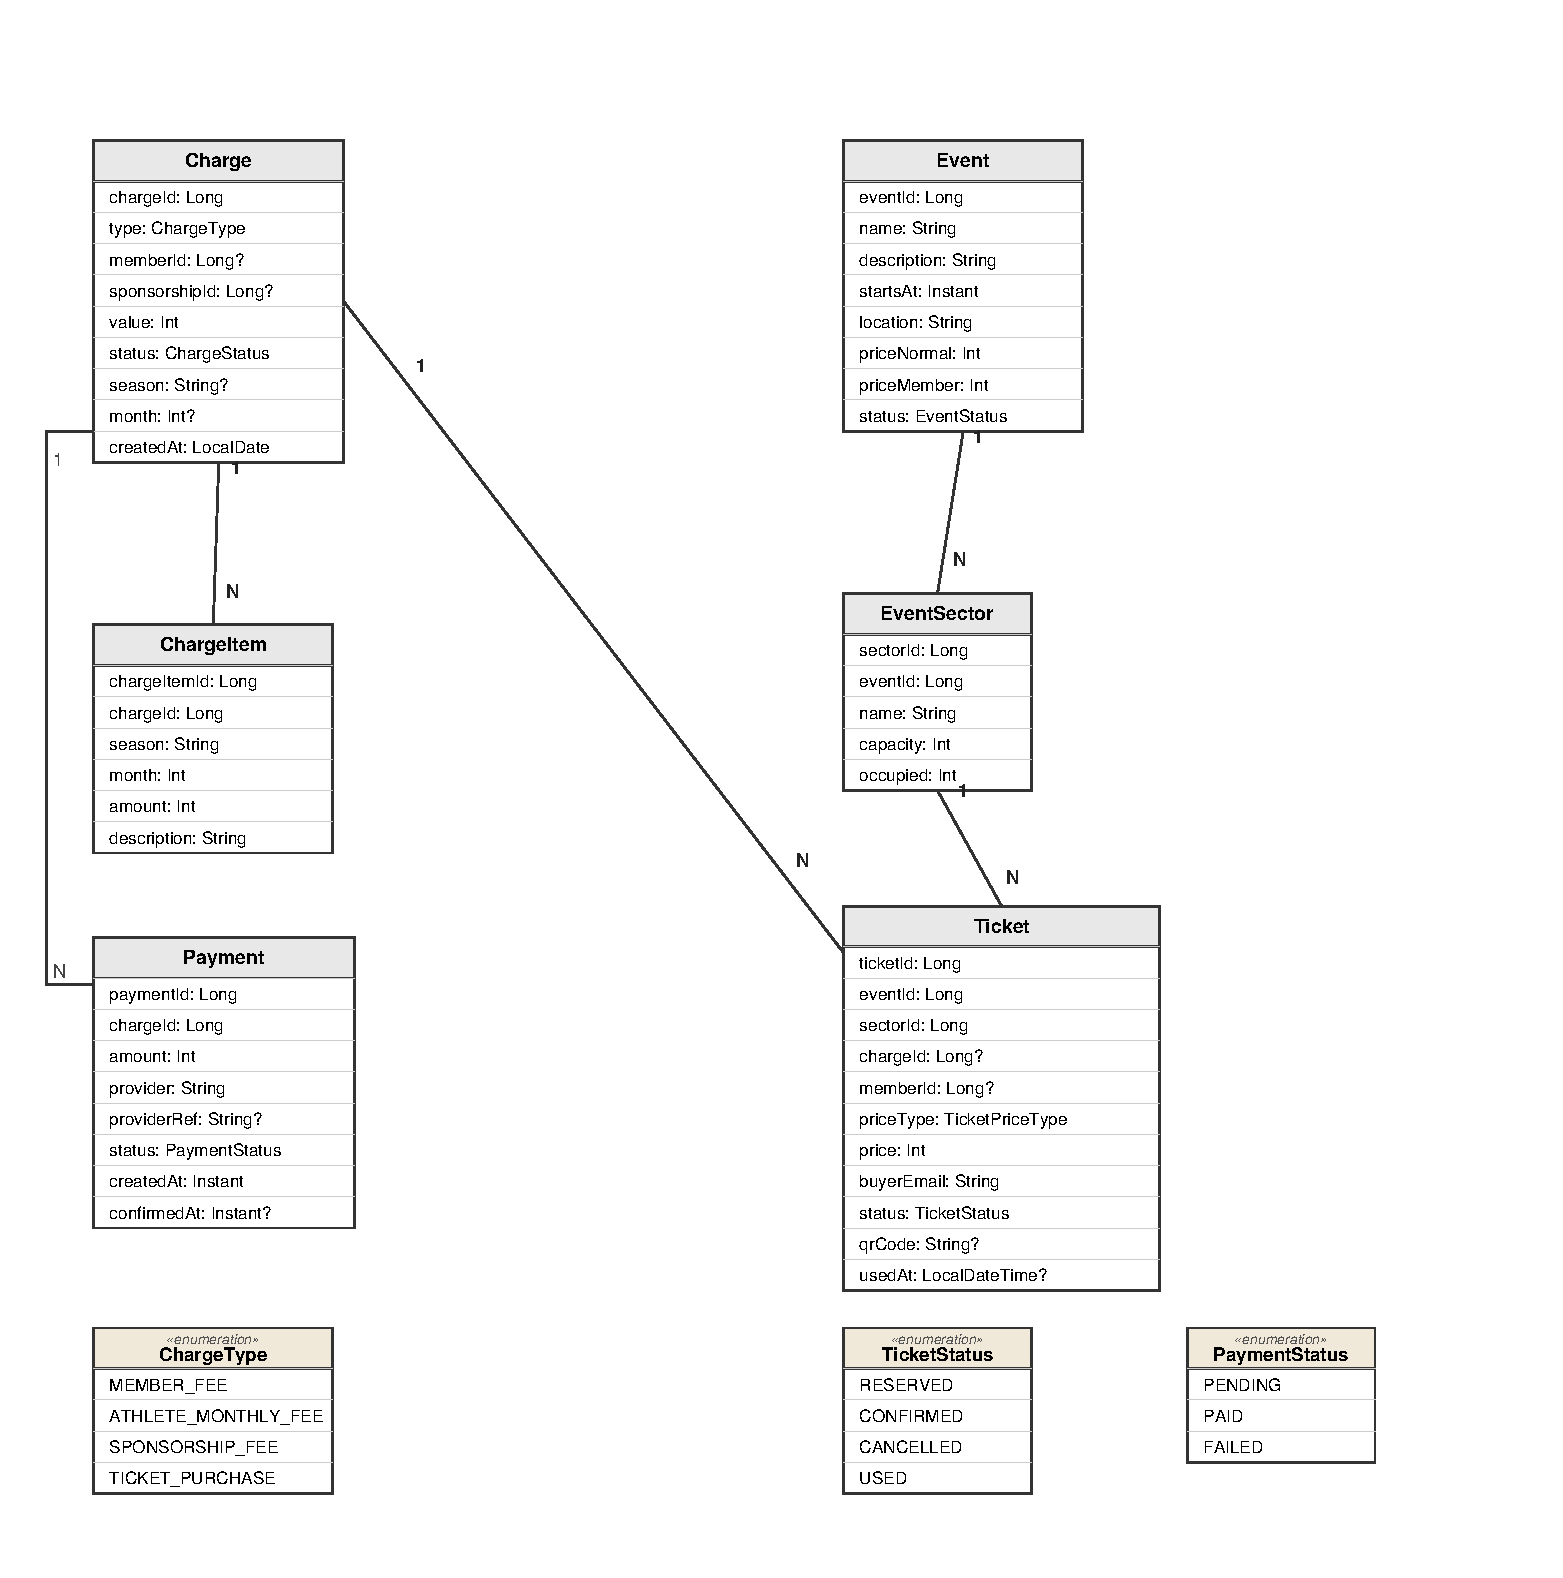
\includegraphics[width=0.85\textwidth]{./figures/er-financas-eventos.pdf}
    \caption{Modelo de dados -- cobranças, pagamentos e eventos}
    \label{fig:er-financas-eventos}
\end{figure}

\subsection{Repositório de Ficheiros}

O repositório de ficheiros é responsável pelo armazenamento de recursos 
binários associados às entidades da aplicação, nomeadamente fotografias de 
perfil, fotografias de sócios e atletas, e documentos como o cartão de cidadão 
ou o exame médico dos atletas.

Importa distinguir dois tipos de informação. Os \textit{metadados} de cada 
ficheiro -- como o nome original, o tipo de conteúdo, o tamanho e a chave de 
armazenamento -- são guardados na base de dados relacional, na entidade 
\texttt{StoredFile}. Já o conteúdo binário dos ficheiros não é guardado na base 
de dados, sendo delegado a um serviço de armazenamento externo, descrito em 
detalhe na Secção~\ref{sec:integracoes}.

Cada ficheiro é identificado por uma chave de armazenamento construída de forma 
hierárquica, que combina o tipo e o identificador da entidade proprietária, o 
tipo de ficheiro e um identificador único. É ainda aplicada uma política de um 
único ficheiro ativo por entidade e tipo, o que significa que o carregamento de 
um novo ficheiro substitui o anterior do mesmo tipo. O carregamento de 
ficheiros está sujeito a validações de tipo e tamanho, distintas consoante se 
trate de imagens ou de documentos.


\section{Serviços}

A camada de serviços é responsável pela lógica de negócio da aplicação. É nela 
que se realiza o processamento dos dados, a aplicação de regras e a 
orquestração das chamadas aos repositórios e aos serviços externos. Cada 
serviço é anotado com \texttt{@Named} e recebe as suas dependências por 
injeção no construtor, e recorre ao \texttt{TransactionManager} para que as 
operações que envolvem múltiplos repositórios sejam executadas no contexto de 
uma única transação.

Todos os serviços seguem uma abordagem de retorno funcional baseada no tipo 
genérico \texttt{Either<L, R>}, que encapsula o sucesso (\texttt{Right}) ou a 
falha (\texttt{Left}) de uma operação. Cada domínio define o seu próprio 
conjunto de erros, o que torna o tratamento de falhas explícito e evita o 
recurso a exceções não controladas. As operações de listagem seguem ainda um 
padrão uniforme de paginação, através das abstrações \texttt{Page} e 
\texttt{PageRequest}.

Existem vários serviços, cada um associado a uma área funcional da aplicação:

\begin{itemize}
    \item \texttt{UserService}: gere os utilizadores e as respetivas sessões, 
    incluindo a criação de utilizadores, a autenticação e a gestão de 
    \textit{tokens};
    \item \texttt{MemberService}: gere o ciclo de vida dos sócios, incluindo a 
    criação, aprovação, rejeição, ativação e desativação, bem como a alteração 
    de dados e de categoria;
    \item \texttt{AthleteService}: gere a inscrição e o ciclo de vida dos 
    atletas. A inscrição de um atleta cria, numa única transação, o sócio 
    associado, o atleta e os respetivos encarregados de educação;
    \item \texttt{EventService}: gere os jogos e a respetiva bilhética, 
    incluindo a criação de eventos e setores e o início do processo de compra 
    de bilhetes;
    \item \texttt{PaymentService}: coordena os pagamentos, as quotas e a 
    emissão de recibos, e integra-se com o serviço de pagamentos externo;
    \item \texttt{SponsorService} e \texttt{SponsorshipService}: gerem, 
    respetivamente, os patrocinadores e os contratos de patrocínio;
    \item \texttt{SponsorshipCatalogService} e \texttt{TeamService}: gerem os 
    catálogos de opções de patrocínio e a organização das equipas e tabelas de 
    preços;
    \item \texttt{AdminOverviewService}: agrega estatísticas para o painel de 
    administração;
    \item \texttt{FileService}: gere o carregamento, a consulta e a remoção de 
    ficheiros, aplicando validações de tipo e tamanho e verificando as 
    permissões de acesso;
    \item \texttt{EmailService}: compõe e envia mensagens de correio 
    eletrónico.
\end{itemize}

A maioria destes serviços segue um modelo simples e consistente: recebem os 
dados, validam as regras de negócio, interagem com os repositórios 
correspondentes e retornam o resultado da operação. Por esse motivo, não são 
detalhados individualmente. O \texttt{PaymentService}, pela sua complexidade e 
pela integração com serviços externos, é descrito em detalhe na 
Secção~\ref{sec:integracoes}.

\section{Controladores}

No contexto da \textit{framework} Spring, um controlador (ou 
\textit{controller}) é o componente responsável por receber e tratar os 
pedidos HTTP efetuados pelos clientes. Estes pedidos são originados a partir da 
aplicação \textit{frontend}, que comunica com o \textit{backend} através de uma 
Web API REST. A função principal de um controlador é interpretar os dados 
recebidos, invocar os serviços adequados e devolver uma resposta apropriada, 
normalmente em formato JSON. Para este efeito, foi utilizada a anotação 
\texttt{@RestController}, apropriada para aplicações que não retornam páginas 
HTML, mas sim dados em formato JSON.

Existem vários controladores na aplicação, cada um responsável por um conjunto 
específico de \textit{endpoints}. Os principais são:

\begin{itemize}
    \item \texttt{UserController}: criação de utilizadores, autenticação 
    (\textit{login} e \textit{logout}) e obtenção da informação do utilizador 
    autenticado;
    \item \texttt{MemberController}: criação, consulta, atualização e gestão do 
    ciclo de vida dos sócios;
    \item \texttt{AthleteController}: inscrição de atletas, consulta pública 
    por escalão e gestão administrativa dos atletas;
    \item \texttt{EventController}: criação e gestão de jogos, consulta de 
    eventos disponíveis e início do processo de compra de bilhetes;
    \item \texttt{PaymentController}: criação de sessões de pagamento, gestão 
    de quotas, emissão de recibos e receção de notificações do serviço de 
    pagamentos;
    \item \texttt{SponsorController} e \texttt{SponsorshipController}: gestão de 
    patrocinadores e de contratos de patrocínio;
    \item \texttt{SponsorshipCatalogController} e \texttt{TeamController}: 
    gestão dos catálogos de patrocínio e da organização das equipas;
    \item \texttt{AdminController}: obtenção de estatísticas para o painel de 
    administração;
    \item \texttt{FileController}: carregamento, consulta e remoção de 
    ficheiros.
\end{itemize}

Importa notar que os controladores que requerem autenticação recebem um objeto 
com a informação do utilizador autenticado, injetado automaticamente pela 
aplicação, como detalhado na Secção~\ref{sec:autenticacao}.

Além da separação clara de responsabilidades, os controladores seguem um 
estilo coeso de tratamento de erros. A aplicação adota o padrão 
\textit{Problem Details for HTTP APIs} (RFC 7807), que devolve 
respostas de erro com uma estrutura unificada em formato JSON, com campos como 
\texttt{type}, \texttt{title}, \texttt{status} e \texttt{detail}, que permitem 
compreender de forma padronizada a natureza do erro ocorrido. A conversão dos 
erros internos de cada domínio para este formato é feita de forma centralizada.

\section{Autenticação e Autorização}
\label{sec:autenticacao}

A autenticação dos utilizadores assenta num mecanismo de \textit{tokens} 
opacos, gerados pela aplicação e persistidos na base de dados. Ao contrário de 
uma palavra-passe, o \textit{token} não transporta qualquer informação 
legível: é apenas uma credencial aleatória que o servidor sabe associar a um 
utilizador. As palavras-passe dos utilizadores nunca são armazenadas em texto 
simples, sendo guardada apenas a sua representação cifrada através do algoritmo 
\textit{BCrypt}.

O processo de autenticação segue os seguintes passos:

\begin{enumerate}
    \item O utilizador submete as suas credenciais (nome de utilizador ou 
    \textit{email}, e palavra-passe);
    \item O servidor procura o utilizador correspondente e valida a 
    palavra-passe submetida contra a representação cifrada armazenada;
    \item Em caso de sucesso, é gerado um \textit{token} aleatório, do qual é 
    guardada na base de dados apenas uma representação cifrada 
    (\textit{hash} SHA-256);
    \item O \textit{token} é devolvido ao cliente, tanto no corpo da resposta 
    como num \textit{cookie} seguro (\texttt{HttpOnly}), utilizado nos pedidos 
    seguintes.
\end{enumerate}

Cada \textit{token} tem associado um tempo de validade absoluto e um tempo de 
validade por inatividade, sendo ainda limitado o número máximo de 
\textit{tokens} ativos por utilizador. A validação dos pedidos autenticados é 
feita de forma centralizada por um \textit{interceptor}, que é executado antes 
dos controladores. Este componente extrai o \textit{token} do cabeçalho de 
autorização (ou, em alternativa, do \textit{cookie}), valida-o e, em caso de 
sucesso, disponibiliza a informação do utilizador autenticado ao controlador. 
Caso a validação falhe, o pedido é rejeitado com o código de estado HTTP 401.

No que diz respeito à autorização, a aplicação define três papéis: 
\texttt{ADMIN}, \texttt{SECRETARIA} e \texttt{NORMAL}. Os papéis 
\texttt{ADMIN} e \texttt{SECRETARIA} partilham o acesso às funcionalidades de 
gestão (\textit{backoffice}), enquanto o papel \texttt{NORMAL} corresponde ao 
utilizador comum. A verificação de permissões é feita ao nível dos serviços e 
dos controladores. Para além da verificação por papel, existe também uma 
verificação de propriedade do recurso, que garante, por exemplo, que um 
utilizador só pode pagar ou consultar dados que lhe dizem respeito.

\section{Integrações Externas}
\label{sec:integracoes}

O \textit{backend} integra-se com vários serviços externos para suportar 
funcionalidades que não fazem parte do seu domínio central. Esta secção 
descreve essas integrações.

\subsection{Pagamentos com Stripe}

O processamento de pagamentos é feito através da plataforma Stripe~\cite{stripe}, 
que trata de toda a interação com os meios de pagamento, sem que os dados 
bancários dos utilizadores passem pelo servidor da aplicação. A integração é 
coordenada pelo \texttt{PaymentService} e suporta diferentes tipos de cobrança: 
quotas de sócio, mensalidades de atleta, patrocínios e compra de bilhetes.

O fluxo de pagamento decorre da seguinte forma:

\begin{enumerate}
    \item O cliente inicia o pagamento através do \textit{endpoint} 
    correspondente;
    \item O \textit{backend} cria a cobrança e os respetivos itens, regista um 
    pagamento no estado pendente e cria uma sessão de pagamento na Stripe, 
    devolvendo ao cliente o endereço para onde deve ser redirecionado;
    \item Após a conclusão do pagamento, a Stripe notifica o \textit{backend} 
    através de um \textit{webhook};
    \item O \textit{backend} valida a autenticidade da notificação e, em caso 
    de sucesso, confirma o pagamento e a cobrança, atualiza o estado das 
    entidades associadas (por exemplo, confirma os bilhetes e gera os 
    respetivos códigos QR) e envia uma mensagem de confirmação ao utilizador. 
    Em caso de falha, o pagamento é marcado como falhado e os recursos 
    reservados são libertados.
\end{enumerate}

A validação da autenticidade das notificações é feita através da verificação de 
uma assinatura, o que impede que pedidos forjados sejam aceites como 
pagamentos válidos.

\subsection{Envio de Correio Eletrónico}

O envio de mensagens de correio eletrónico é suportado pelo módulo de 
\textit{email} do Spring, configurado para comunicar com um servidor SMTP 
externo. A composição das mensagens é da responsabilidade do 
\texttt{EmailService}, que gera conteúdo em HTML. A principal utilização atual 
é o envio da confirmação de compra de bilhetes, na qual os códigos QR são 
incluídos como imagens incorporadas na própria mensagem.

\subsection{Armazenamento de Ficheiros}

O conteúdo binário dos ficheiros não é guardado na base de dados, mas sim num serviço de armazenamento 
externo. A aplicação utiliza o serviço Cloudflare R2, acedido através de uma 
API compatível com o protocolo S3 da Amazon. O acesso ao armazenamento é 
abstraído por uma interface, o que permite, no futuro, substituir o serviço 
utilizado sem alterar a lógica da aplicação. Este serviço é utilizado para 
armazenar fotografias de perfil, fotografias de sócios e atletas, e documentos 
associados aos atletas.

\subsection{Geração de Códigos QR}

A geração dos códigos QR utilizados na bilhética é feita através da biblioteca 
ZXing~\cite{zxing}. A partir de um identificador único associado a cada 
bilhete, é gerada uma imagem que é posteriormente incluída na mensagem de 
confirmação de compra enviada ao utilizador.

% Capitulo 5
\chapter{Frontend}

O \textit{frontend} da aplicação tem como principal objetivo fornecer uma 
interface intuitiva e interativa para que os utilizadores possam aceder às 
funcionalidades do clube, nomeadamente a adesão de sócios, a inscrição de 
atletas, o registo de patrocínios e a compra de bilhetes, bem como permitir a 
gestão destas áreas por parte dos utilizadores responsáveis.

Esta interface é construída como uma SPA (\textit{Single Page 
Application}), ou seja, uma aplicação de página única, na qual a 
navegação entre as diferentes secções não implica o recarregamento da página. 
Foi desenvolvida na linguagem TypeScript, uma linguagem 
fortemente tipificada que se baseia em JavaScript e que permite uma maior 
segurança em tempo de desenvolvimento e a deteção antecipada de erros. Para a 
construção da interface foi utilizada a biblioteca React~\cite{react}, que 
permite a construção de interfaces baseadas em componentes reutilizáveis, com 
atualização e renderização eficientes através de uma DOM virtual.

O empacotamento e o ambiente de desenvolvimento são geridos pela ferramenta 
Vite~\cite{vite}, que oferece um servidor de desenvolvimento rápido e um 
processo de \textit{build} otimizado. Durante o desenvolvimento, o Vite está 
ainda configurado para reencaminhar os pedidos dirigidos à API para o servidor 
do \textit{backend}, o que simplifica a comunicação entre as duas componentes.

No que diz respeito ao aspeto visual, a aplicação combina duas abordagens. Por 
um lado, recorre ao Tailwind CSS~\cite{tailwind}, uma \textit{framework} de CSS 
utilitária que define um tema próprio (paleta de cores, tipografia e animações) 
alinhado com a identidade visual do clube. Por outro, utiliza folhas de estilo 
de CSS próprias, organizadas por funcionalidade, para os estilos mais 
específicos de cada área da aplicação.

\section{Estrutura da Aplicação}

A aplicação está organizada de forma modular, separada por domínio funcional. 
O código divide-se em duas grandes áreas: uma pasta de código transversal, 
partilhado por toda a aplicação, e uma pasta de funcionalidades, na qual cada 
domínio (atletas, sócios, patrocínios, eventos, utilizadores, entre outros) 
constitui uma unidade autocontida.

Cada funcionalidade agrupa os seus próprios componentes, tipos de dados, 
estilos, lógica de orquestração e o acesso à API. Esta organização mantém 
próximos todos os elementos relativos a uma mesma área, o que facilita a 
manutenção e a evolução do código. Entre os elementos transversais, partilhados 
por todas as funcionalidades, incluem-se componentes reutilizáveis (como o 
cabeçalho, o rodapé e os campos de formulário), funções utilitárias, a 
configuração da aplicação e a gestão da autenticação.

A comunicação com o \textit{backend} é feita através de uma camada de acesso à 
Web API, separada por entidade. Cada funcionalidade define as operações de que 
necessita sobre uma função auxiliar comum, que efetua os pedidos HTTP, inclui 
as credenciais de sessão e converte as respostas de erro do servidor numa 
exceção uniforme. Desta forma, os componentes consomem funções bem definidas 
em vez de lidarem diretamente com os detalhes da comunicação em rede.

A lógica de cada área é frequentemente encapsulada em \textit{hooks} 
personalizados, que combinam o carregamento de dados a partir do 
\textit{backend} com a gestão do estado da interface. Esta abordagem baseada em 
\textit{hooks} permite uma estrutura declarativa, na qual a interface reflete o 
estado da aplicação a cada momento.

\section{Navegação e Autenticação}

A navegação entre as páginas da aplicação é gerida pela biblioteca React 
Router~\cite{reactrouter}, que define as rotas da aplicação num único ponto e 
permite a composição de \textit{layouts} reutilizáveis partilhados por várias 
páginas.

O estado de autenticação do utilizador é mantido de forma global através do 
mecanismo de contexto do React. Ao iniciar, a aplicação consulta o 
\textit{backend} para determinar se existe uma sessão ativa e, em caso 
afirmativo, carrega a informação do utilizador autenticado, que fica acessível 
a toda a aplicação. A sessão é suportada por \textit{cookies} geridos pelo 
\textit{backend}, enviados automaticamente em todos os pedidos.

A aplicação adapta-se ao papel do utilizador autenticado (\texttt{ADMIN}, 
\texttt{SECRETARIA} ou \texttt{NORMAL}). Esta adaptação ocorre a dois níveis. 
Ao nível da navegação, as rotas são protegidas por componentes que verificam, 
antes de apresentar uma página, se o utilizador está autenticado e se possui o 
papel necessário, redirecionando-o caso contrário. Toda a área de gestão 
(\textit{backoffice}) está protegida desta forma, acessível apenas a 
utilizadores com os papéis \texttt{ADMIN} ou \texttt{SECRETARIA}. Ao nível da 
interface, vários elementos são apresentados condicionalmente consoante o papel 
do utilizador, como por exemplo as ligações para a área de gestão ou os campos 
adicionais disponíveis apenas aos responsáveis do clube.

\section{Interface da Aplicação}

A aplicação apresenta uma navegação simples entre as principais áreas, através 
de um menu superior. Podem distinguir-se duas grandes vertentes: uma área 
pública, orientada para o visitante e para o sócio, e uma área de gestão, 
orientada para os utilizadores responsáveis pela administração do clube.

Na área pública encontram-se a página inicial, os fluxos de adesão de sócio, 
inscrição de atleta e registo de patrocínio, a consulta de atletas por escalão 
e a compra de bilhetes para os jogos. Na área de gestão é possível consultar e 
gerir sócios, atletas, patrocínios e eventos, administrar os utilizadores da 
aplicação e configurar os catálogos de opções e as tabelas de preços. Esta 
área dispõe ainda de um painel inicial com estatísticas gerais sobre o estado 
do clube.

\section{Comunicação com a API}

A comunicação entre o \textit{frontend} e o \textit{backend} é realizada através
de pedidos HTTP para a Web API REST disponibilizada pelo servidor. Para
centralizar esta comunicação, cada domínio funcional possui o seu próprio
ficheiro de acesso à API, como por exemplo \texttt{auth/api.ts},
\texttt{Members/api.ts}, \texttt{Athletes/api.ts}, \texttt{sponsors/api.ts},
\texttt{events/api.ts}, \texttt{files/api.ts} e \texttt{admin/api.ts}.

Apesar de cada funcionalidade definir as operações específicas de que necessita,
a estrutura dos pedidos segue um padrão comum. O endereço base da API é definido
num ficheiro de configuração partilhado, através da constante \texttt{BASE\_URL},
cujo valor é \texttt{/api}. Desta forma, os componentes da aplicação não
dependem diretamente do endereço absoluto do servidor, o que facilita a execução
em diferentes ambientes, como desenvolvimento local ou Docker.

Durante o desenvolvimento, o servidor Vite reencaminha automaticamente os
pedidos feitos para \texttt{/api} para o servidor do \textit{backend}. Este
mecanismo de \textit{proxy} evita problemas de CORS (\textit{Cross-Origin
Resource Sharing}) e permite que o \textit{frontend} comunique com o
\textit{backend} como se ambos estivessem disponíveis no mesmo domínio.

Todos os pedidos autenticados incluem a opção \texttt{credentials: "include"},
permitindo que os \textit{cookies} de sessão definidos pelo \textit{backend}
sejam enviados automaticamente. Esta decisão mantém a lógica de autenticação
centrada no servidor, reduzindo a necessidade de manipulação manual de tokens no
\textit{frontend}.

O tratamento de erros também segue uma abordagem uniforme. Quando uma resposta
da API indica erro, a camada de acesso converte essa resposta numa exceção ou
num objeto de erro coerente, que é posteriormente tratado pelos componentes ou
pelos \textit{hooks}. Esta abordagem evita que cada componente tenha de
interpretar manualmente códigos HTTP e formatos de erro diferentes.

\section{Gestão de Estado e Hooks}

A aplicação utiliza o estado local do React para gerir a informação necessária
em cada componente, como valores de formulários, mensagens de erro, estados de
carregamento e resultados de operações. Para evitar duplicação de lógica, foram
criados vários \textit{hooks} personalizados, organizados por funcionalidade.

Estes \textit{hooks} encapsulam operações como o carregamento de listas, a
consulta de detalhes, a criação e atualização de entidades e a execução de ações
administrativas. Por exemplo, existem \textit{hooks} para carregar sócios,
consultar detalhes de um atleta, gerir catálogos de patrocínio, obter
estatísticas de administração ou consultar eventos.

Esta organização traz várias vantagens:

\begin{itemize}
    \item separa a lógica de carregamento de dados da lógica visual dos
    componentes;
    \item reduz a repetição de código entre páginas semelhantes;
    \item torna os componentes mais declarativos e fáceis de compreender;
    \item facilita a manutenção, uma vez que alterações na forma de comunicar
    com a API ficam concentradas nos \textit{hooks} ou nos ficheiros de API.
\end{itemize}

Além dos \textit{hooks} específicos de cada domínio, existem também
\textit{hooks} partilhados, como \texttt{useAuth}, utilizado para aceder ao
estado global de autenticação, e \texttt{useStatusHandler}, utilizado para
tratar estados comuns de operações assíncronas, como carregamento, sucesso e
erro.

\section{Componentes Reutilizáveis}

A aplicação recorre a vários componentes reutilizáveis, localizados na pasta
\texttt{shared/components}. Estes componentes representam elementos comuns da
interface, utilizados em várias áreas da aplicação.

Entre os principais componentes partilhados destacam-se:

\begin{itemize}
    \item \texttt{Header}: cabeçalho da aplicação, responsável pela navegação
    principal e pela apresentação de opções dependentes do estado de
    autenticação;
    \item \texttt{Footer}: rodapé da aplicação, contendo informação institucional
    e ligações relevantes;
    \item \texttt{Require} e \texttt{AuthRequire}: componentes responsáveis por
    proteger rotas de acordo com o estado de autenticação e o papel do
    utilizador;
    \item \texttt{Form}: componente auxiliar para estruturar formulários;
    \item \texttt{LabeledField}: componente utilizado para apresentar campos com
    rótulo de forma consistente;
    \item \texttt{MessageFormBox}: componente utilizado para apresentar mensagens
    de erro, sucesso ou informação ao utilizador.
\end{itemize}

A existência destes componentes contribui para uma interface mais consistente e
reduz a repetição de código. Por exemplo, os formulários de criação e edição de
sócios ou atletas partilham padrões visuais e comportamentais semelhantes,
permitindo ao utilizador reconhecer rapidamente a forma de interação esperada.

\section{Rotas da Aplicação}

A navegação da aplicação é definida de forma centralizada no ficheiro
\texttt{jagozRouter.tsx}, através da função \texttt{createBrowserRouter} da
biblioteca React Router. Esta configuração descreve todas as páginas
disponíveis e a forma como estão organizadas.

As principais rotas públicas incluem:

\begin{itemize}
    \item \texttt{/}: página inicial da aplicação;
    \item \texttt{/auth/login}: página de autenticação;
    \item \texttt{/auth/register}: página de registo de utilizador;
    \item \texttt{/athletes/category/:teamCategory}: listagem pública de atletas
    por escalão;
    \item \texttt{/athletes/:athleteId}: perfil público de um atleta;
    \item \texttt{/sponsors/info}: página informativa sobre patrocínios;
    \item \texttt{/tickets}: listagem pública de eventos disponíveis para compra
    de bilhetes;
    \item \texttt{/tickets/:eventId}: fluxo de compra de bilhetes para um evento.
\end{itemize}

Existem também rotas protegidas, acessíveis apenas a utilizadores autenticados,
como:

\begin{itemize}
    \item \texttt{/profile}: perfil do utilizador autenticado;
    \item \texttt{/members/create}: adesão ou criação de sócio;
    \item \texttt{/athletes/register}: inscrição de atleta;
    \item \texttt{/sponsors/create}: criação de pedido de patrocínio;
    \item \texttt{/sponsors/my}: consulta dos patrocínios associados ao
    utilizador.
\end{itemize}

Por fim, a área de administração encontra-se agrupada sob a rota
\texttt{/admin}. Esta área é protegida por componentes de autorização e apenas
pode ser acedida por utilizadores com os papéis \texttt{ADMIN} ou
\texttt{SECRETARIA}.

\begin{itemize}
    \item \texttt{/admin}: Painel inicial de administração;
    \item \texttt{/admin/members}: Gestão de sócios;
    \item \texttt{/admin/athletes}: Gestão de atletas;
    \item \texttt{/admin/users}: Gestão de utilizadores;
    \item \texttt{/admin/sponsors}: Gestão de patrocínios;
    \item \texttt{/admin/events}: Gestão de eventos;
    \item \texttt{/admin/team-settings}: Configuração de equipas e escalões;
\end{itemize}

Para além destas rotas principais, existem rotas auxiliares para operações
específicas, como criação, edição e consulta de detalhe. Por exemplo, a gestão
de sócios inclui rotas para criar um novo sócio, consultar o detalhe de um
sócio existente e editar os seus dados. Esta organização evita concentrar todas
as operações numa única página e permite separar claramente cada fluxo de
utilização.

\section{Funcionalidades por Domínio}

O \textit{frontend} encontra-se organizado por funcionalidades, cada uma
representando uma área do sistema. Esta organização permite que cada domínio
tenha os seus próprios componentes, tipos, estilos, \textit{hooks} e chamadas à
API.

\subsection{Página Inicial}

A página inicial funciona como ponto de entrada da aplicação. Apresenta a
identidade visual do clube, uma área de destaque e secções informativas, como
notícias e classificações. Esta página tem uma função essencialmente pública,
servindo para orientar visitantes e utilizadores para as principais ações
disponíveis, como inscrição, consulta de atletas, patrocínios e compra de
bilhetes.

A componente visual desta página utiliza imagens públicas do clube e estilos
próprios, definidos na funcionalidade \texttt{home}. Esta área inclui
componentes como \texttt{Hero}, \texttt{NewsGrid} e \texttt{StandingTable}.

 \begin{figure}[H]
    \centering
    
    
\includegraphics[width=\textwidth]{./figures/frontend-HomePage.png}
    \caption{Página inicial da aplicação}
    \label{fig:frontend-HomePage}
\end{figure}

\subsection{Autenticação}

A funcionalidade de autenticação inclui as páginas de início de sessão e de
registo. O início de sessão permite ao utilizador autenticar-se com as suas
credenciais, recebendo do \textit{backend} uma sessão válida. Após autenticação,
a informação do utilizador é guardada no contexto global da aplicação.

O registo permite criar uma nova conta de utilizador. Esta conta pode depois
ser associada a um sócio, atleta ou patrocinador, dependendo do fluxo de
utilização. Esta separação entre conta de utilizador e entidades do clube
permite maior flexibilidade, uma vez que nem todos os utilizadores são
necessariamente sócios ou patrocinadores no momento da criação da conta.

\begin{figure}[H]
    \centering
    
    
\includegraphics[width=\textwidth]{./figures/frontend-LoginPage.png}
    \caption{Página de autenticação}
    \label{fig:frontend-LoginPage}
\end{figure}

\subsection{Sócios}

A área de sócios permite criar, consultar, editar e gerir sócios do clube. No
lado público ou autenticado, o utilizador pode preencher o formulário de adesão,
introduzindo dados pessoais, contactos, morada, NIF, categoria e consentimentos.

Na área administrativa, os utilizadores com permissões podem consultar a lista
de sócios, aplicar filtros, aceder ao detalhe de cada sócio e executar ações de
gestão, como aprovação, rejeição, reativação, alteração de categoria ou edição
dos dados.

Esta funcionalidade inclui também a apresentação de informação financeira
associada ao sócio, nomeadamente quotas ou pagamentos pendentes, quando
aplicável. O acesso a recibos é feito através de ligações para os
\textit{endpoints} de pagamento disponibilizados pelo \textit{backend}.

\begin{figure}[H]
    \centering
    
    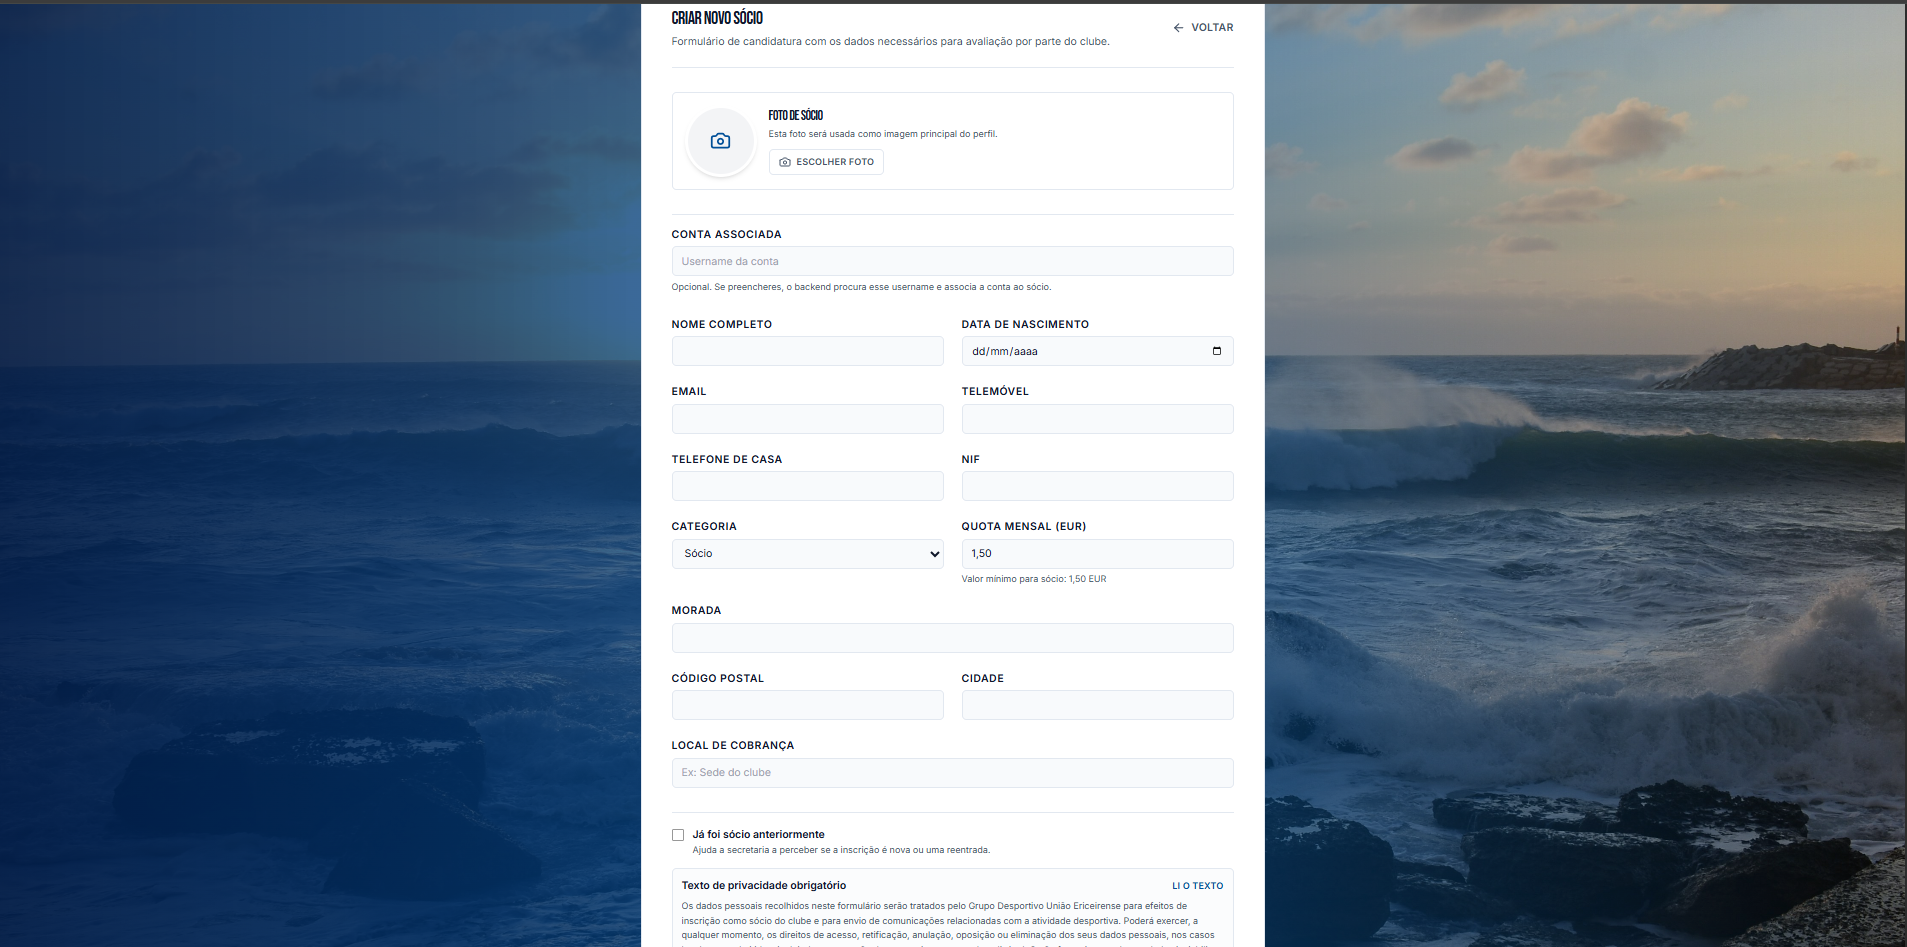
\includegraphics[width=\textwidth]{./figures/frontend-MemberFormPage.png}
    \caption{Formulário de adesão de sócio}
    \label{fig:frontend-MemberFormPage}
\end{figure}

\subsection{Atletas}

A funcionalidade de atletas suporta dois tipos principais de utilização. Por um
lado, permite a inscrição de novos atletas através de um formulário detalhado.
Este formulário recolhe dados pessoais, informação desportiva, dados escolares,
informação médica/administrativa e dados dos encarregados de educação.

Por outro lado, permite a consulta pública de atletas por escalão. Esta
consulta expõe apenas informação não sensível, como nome, número, posição,
nacionalidade, idade e escalão. Dados sensíveis, como documentos, contactos,
NIF, número de identificação ou dados de encarregados de educação, ficam
reservados à área administrativa.

Na área de gestão, os responsáveis podem consultar todos os atletas, incluindo
pendentes e rejeitados, editar dados administrativos, alterar o escalão,
aprovar ou rejeitar inscrições e ativar ou desativar atletas.

Existe ainda uma página de configuração de equipas, onde é possível gerir
grupos, escalões e tabelas de preços utilizadas nas opções de patrocínio
associadas a equipas.

\begin{figure}[H]
    \centering
    
    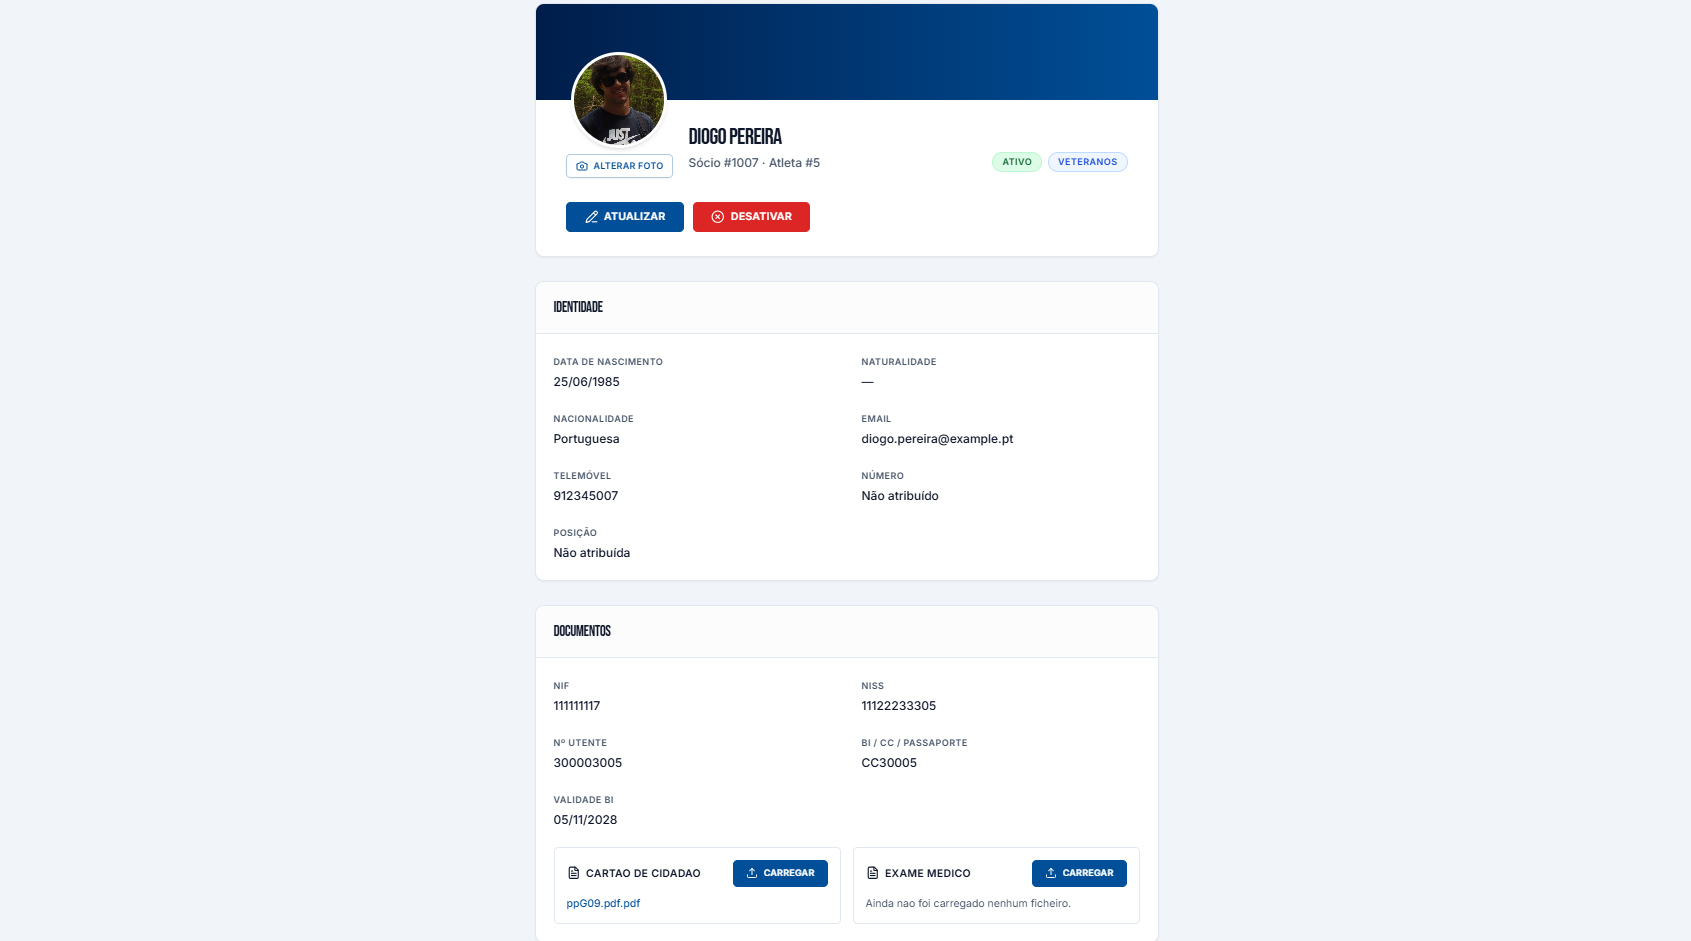
\includegraphics[width=\textwidth]{./figures/frontend-AthleteProfilePage.png}
    \caption{Página de perfil de atleta}
    \label{fig:frontend-AthleteProfilePage}
\end{figure}

\subsection{Patrocínios}

A área de patrocínios permite que um utilizador consulte informação sobre as
opções disponíveis e submeta um pedido de patrocínio. O sistema suporta
diferentes tipos de patrocínio, como publicidade em lona/outdoor, patrocínio de
equipas e apoio a outras modalidades ou iniciativas.

O \textit{frontend} apresenta os catálogos de opções disponíveis, calcula os
valores associados e permite a submissão do pedido. Para utilizadores
autenticados, existe também uma área de consulta dos seus próprios patrocínios,
onde podem acompanhar o estado de cada pedido e aceder aos detalhes ou recibos.

Na área administrativa, os responsáveis podem consultar todos os patrocínios,
aprovar pedidos, marcar pagamentos, cancelar contratos, gerir patrocinadores e
configurar os catálogos de opções. Esta configuração inclui opções de
publicidade, colocações em equipamentos, outras modalidades e regras de preços
por grupo ou escalão.

\begin{figure}[H]
    \centering
    
    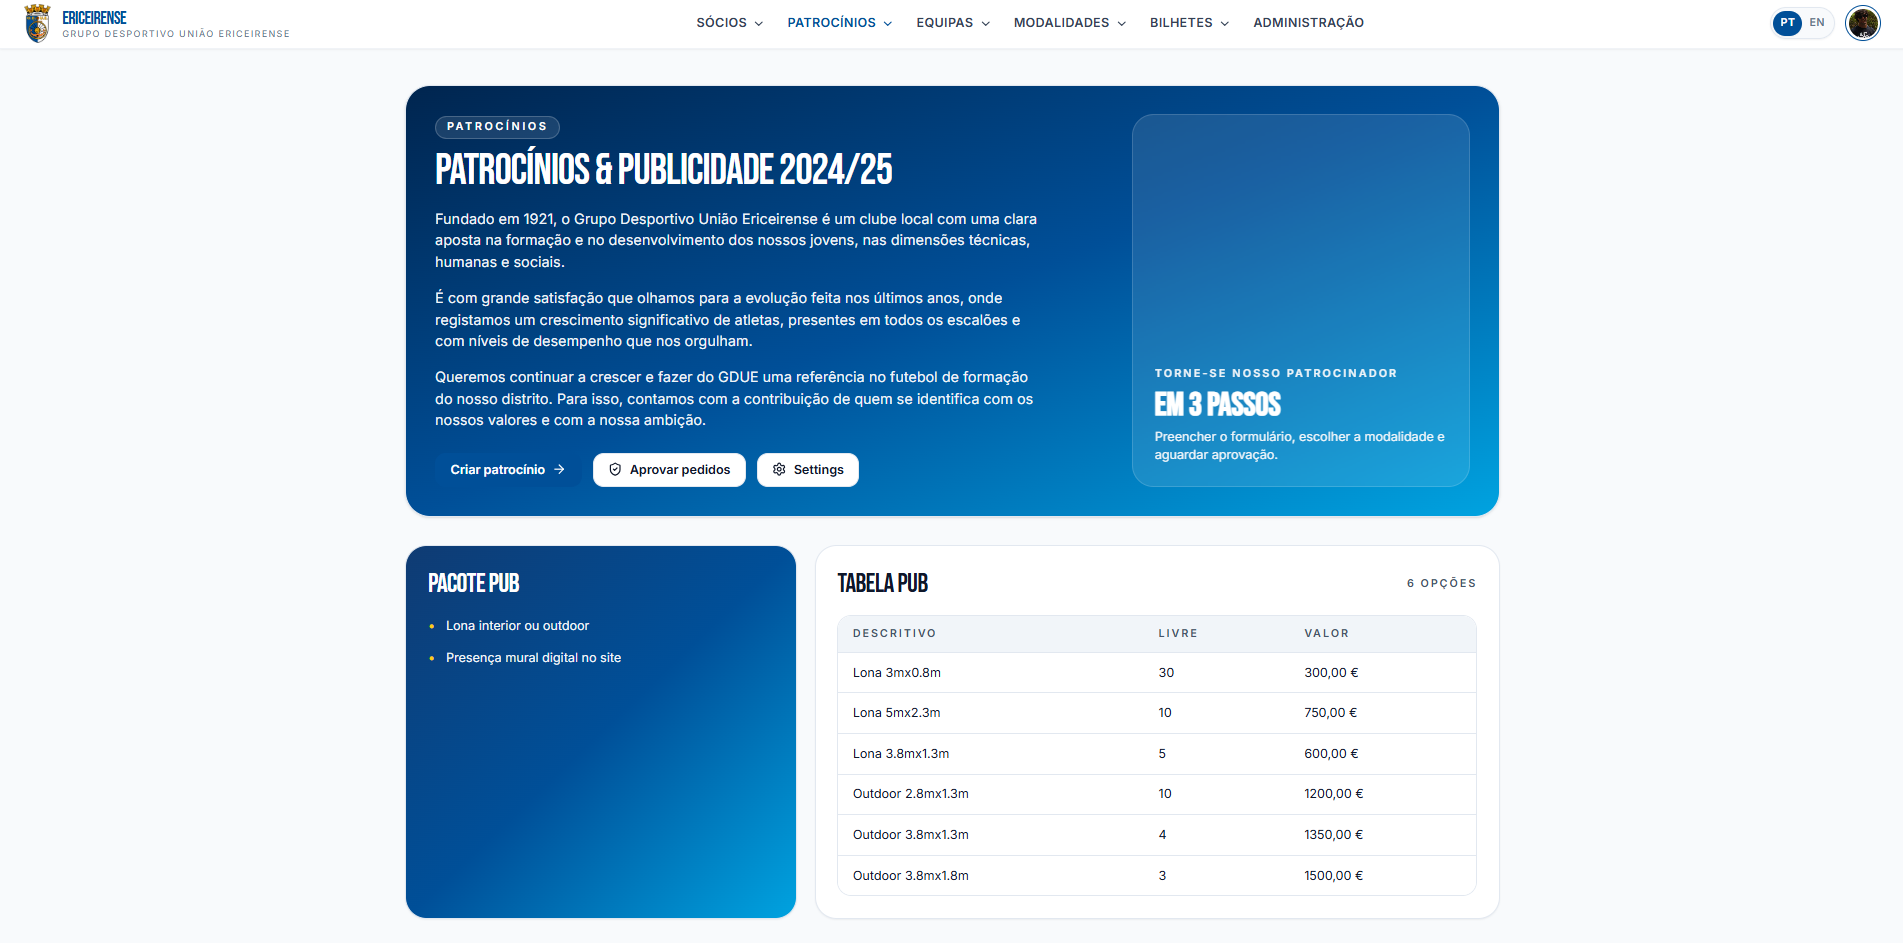
\includegraphics[width=\textwidth]{./figures/frontend-SponsorInfoPage.png}
    \caption{Página de Informação sobre Patrocínios}
    \label{fig:frontend-SponsorInfoPage}
\end{figure}

\subsection{Eventos e Bilheteira}

A funcionalidade de eventos permite criar e gerir jogos ou outros eventos do
clube. Na área administrativa, é possível criar eventos, definir descrição,
local, data, preços para público geral e sócios, e configurar setores com
lotação própria.

A área pública de bilheteira permite consultar eventos disponíveis e iniciar o
processo de compra de bilhetes. Durante este processo, o utilizador seleciona
os setores pretendidos e informa os dados necessários para a compra. Quando o
bilhete é de sócio, o sistema suporta a validação do número de sócio e da data
de nascimento, garantindo que o desconto é aplicado apenas a sócios válidos.

Após a criação da sessão de pagamento, o utilizador é redirecionado para o
serviço de pagamento. O \textit{frontend} possui ainda páginas específicas para
o resultado do pagamento, nomeadamente sucesso e cancelamento, acessíveis pelas
rotas \texttt{/payments/success} e \texttt{/payments/cancel}.

\subsection{Utilizadores e Perfil}

A área de utilizadores permite ao utilizador autenticado consultar o seu perfil
e as entidades a si associadas, como sócio, atleta ou patrocinadores. Na área
administrativa, os responsáveis podem consultar a lista de utilizadores, aceder
ao detalhe de cada um, alterar o papel atribuído e associar um sócio ativo.

Esta funcionalidade é importante para ligar a autenticação às entidades do
domínio do clube. Um utilizador pode ter permissões diferentes consoante o seu
papel, mas também pode estar associado a um sócio ou patrocinador, o que
influencia as ações que pode realizar.

\subsection{Ficheiros}

A aplicação inclui uma funcionalidade dedicada à gestão de ficheiros, utilizada
por várias áreas do sistema. Esta funcionalidade permite listar, carregar,
consultar e remover ficheiros associados a entidades como utilizadores, sócios
ou atletas.

No \textit{frontend}, esta gestão é encapsulada em componentes e funções de API
próprias. Os ficheiros são enviados através de pedidos
\texttt{multipart/form-data}, adequados ao envio de conteúdo binário. Para
visualização ou acesso aos ficheiros, a aplicação constrói ligações para os
\textit{endpoints} do \textit{backend}, como o conteúdo de um ficheiro ou a
fotografia pública de um atleta.

A utilização desta funcionalidade permite manter a gestão documental integrada
na aplicação, sem misturar o conteúdo binário com os dados estruturados
apresentados nos formulários.

\subsection{Administração}

A área de administração funciona como o \textit{backoffice} da aplicação. O seu
acesso está reservado a utilizadores com os papéis \texttt{ADMIN} ou
\texttt{SECRETARIA}. Esta área reúne as ferramentas necessárias para gerir o
funcionamento do clube.

O painel inicial apresenta estatísticas gerais, permitindo obter uma visão
rápida sobre o estado da organização, como número de sócios, atletas,
patrocínios ou pedidos pendentes. A partir deste painel, os responsáveis podem
navegar para as diferentes áreas de gestão: sócios, atletas, utilizadores,
patrocínios, eventos e configurações.

\begin{figure}[H]
    \centering
    
    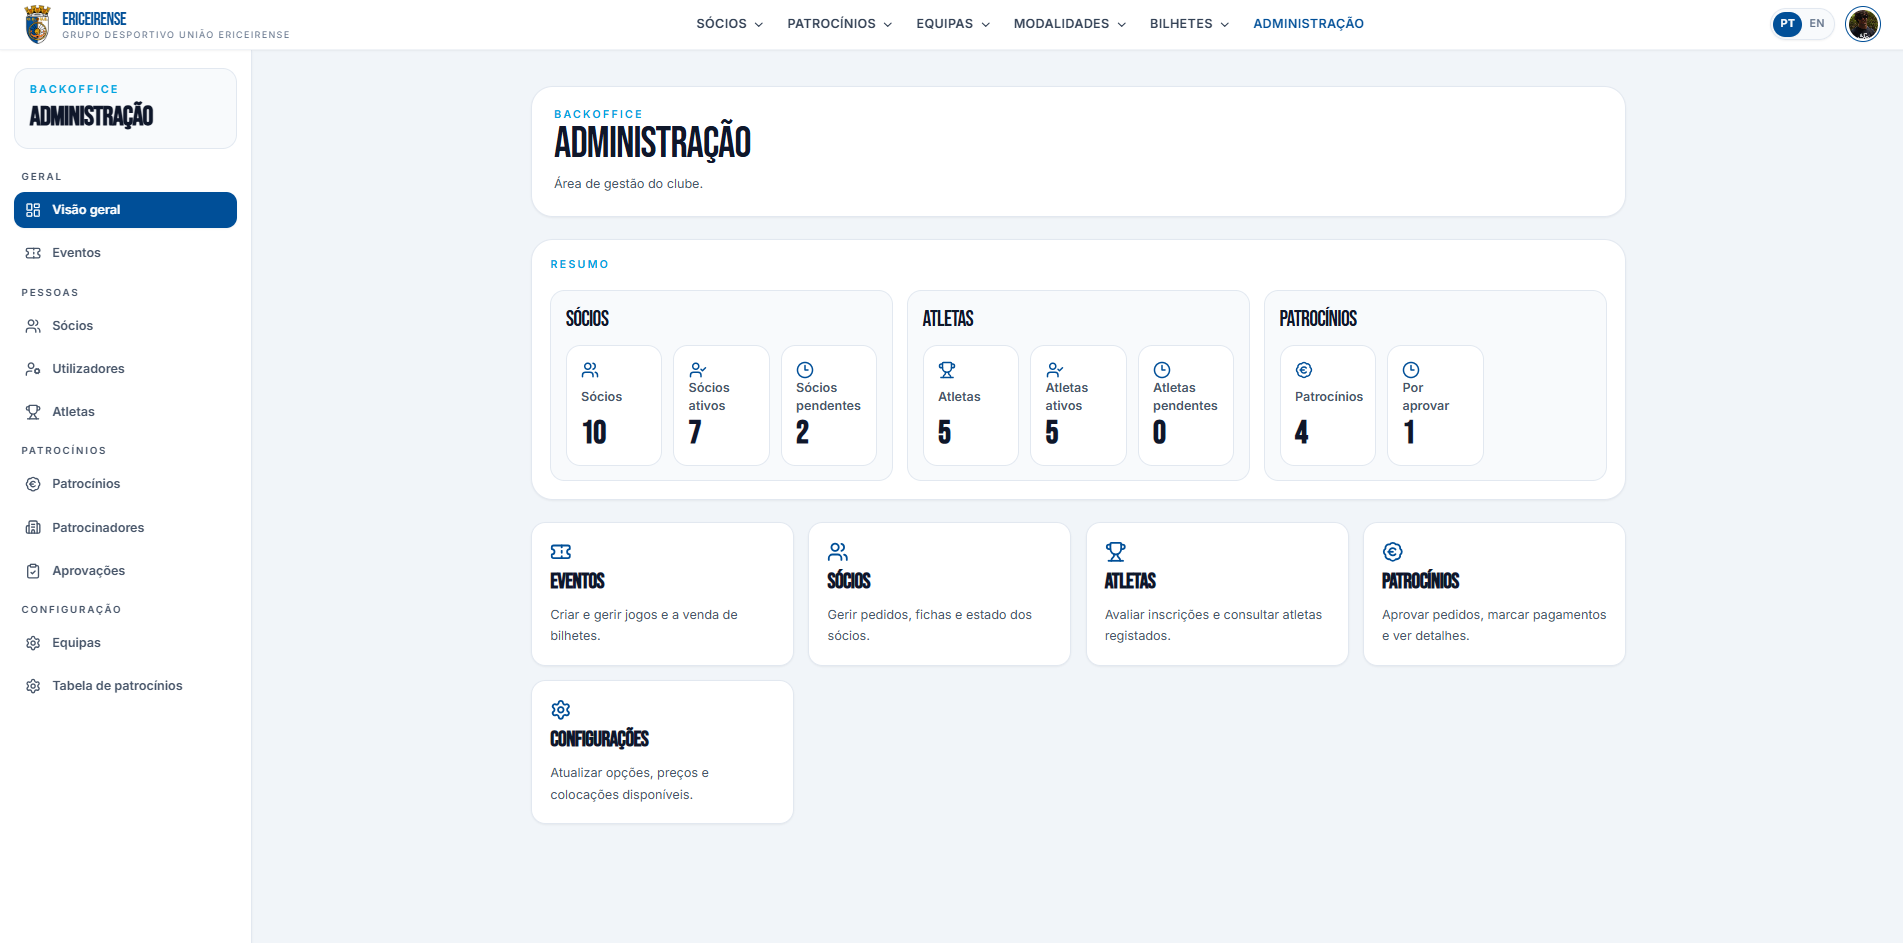
\includegraphics[width=\textwidth]{./figures/frontend-AdminPage.png}
    \caption{Página Inicial do BackOffice}
    \label{fig:frontend-AdminPage}
\end{figure}

\section{Formulários e Validação}

Uma parte significativa da aplicação é composta por formulários, uma vez que os
principais processos do clube envolvem recolha de dados: adesão de sócios,
inscrição de atletas, criação de patrocínios, edição de utilizadores e criação
de eventos.

Os formulários são estruturados em componentes específicos, como
\texttt{MemberForm} e \texttt{AthleteForm}, e utilizam tipos TypeScript para
representar os dados esperados. Para facilitar a inicialização e transformação
dos valores dos formulários, existem ficheiros utilitários como
\texttt{formValues.ts}, que concentram valores por omissão e conversões
necessárias antes do envio para a API.

A validação é feita em dois níveis. No \textit{frontend}, são aplicadas
validações imediatas que melhoram a experiência do utilizador, como campos
obrigatórios, formatos de datas, valores numéricos e conversões monetárias. No
\textit{backend}, as regras de negócio são novamente validadas, garantindo que
a integridade dos dados não depende apenas da interface.

Esta dupla validação é importante porque o \textit{frontend} melhora a
usabilidade, mas o \textit{backend} continua a ser a fonte de verdade das
regras da aplicação.

\section{Tipos e Segurança em Tempo de Desenvolvimento}

A utilização de TypeScript permite declarar tipos para os dados manipulados
pela aplicação. Cada funcionalidade define os seus próprios tipos, como
\texttt{Member}, \texttt{Athlete}, \texttt{Sponsorship}, \texttt{Event} ou
tipos auxiliares de formulários.

Esta tipagem contribui para reduzir erros durante o desenvolvimento. Por
exemplo, se uma função espera um identificador numérico ou um determinado
campo obrigatório, o compilador consegue assinalar usos incorretos antes da
execução da aplicação. Isto torna o código mais previsível e facilita a
refatoração.

A tipagem é especialmente útil na comunicação com a API, uma vez que as
respostas do \textit{backend} são convertidas para estruturas conhecidas no
\textit{frontend}. Embora esta validação não substitua a validação no servidor,
ajuda a manter consistência entre as duas camadas.

\section{Tratamento de Estados da Interface}

As operações assíncronas, como carregamento de listas, submissão de formulários
ou atualização de dados, exigem a representação de diferentes estados na
interface. A aplicação distingue estados como carregamento, sucesso, erro e
ausência de dados.

Esta distinção permite fornecer uma experiência mais clara ao utilizador. Por
exemplo, durante o carregamento de uma lista, a interface pode apresentar uma
mensagem ou indicador de espera; em caso de erro, pode mostrar uma mensagem
descritiva; e após uma operação bem-sucedida, pode redirecionar o utilizador ou
apresentar confirmação.

A existência de funções e \textit{hooks} auxiliares para este tratamento evita
que cada componente implemente de forma diferente a mesma lógica de estado.

\section{Estilo Visual e Responsividade}

O estilo visual da aplicação combina CSS próprio com Tailwind CSS. As folhas de
estilo específicas de cada funcionalidade permitem controlar detalhes visuais
de páginas complexas, como formulários, painéis de administração, cartões,
listas e tabelas. O Tailwind CSS é utilizado como base utilitária e para
definir um tema coerente.

A aplicação procura refletir a identidade visual do clube, recorrendo a imagens
e elementos gráficos presentes na pasta pública, como o logótipo e imagens de
fundo. Estes elementos ajudam a aproximar a interface da identidade institucional
do GDUE.

A responsividade é uma preocupação importante, uma vez que a aplicação pode ser
utilizada tanto em computadores como em dispositivos móveis. A interface é
organizada para se adaptar a diferentes larguras de ecrã, especialmente nas
áreas públicas, como a página inicial, consulta de atletas, inscrição e compra
de bilhetes. Nas áreas administrativas, onde existe maior densidade de
informação, a prioridade é manter a leitura clara e a navegação eficiente.

\section{Internacionalização}

Uma das funcionalidades relevantes do \textit{frontend} é o suporte a múltiplos
idiomas, através de um módulo de internacionalização (i18n). Esta funcionalidade
foi considerada importante no contexto do clube, uma vez que a Ericeira conta
atualmente com uma comunidade internacional significativa: o clube integra
cerca de 20 nacionalidades diferentes, na sua maioria sem o português como
língua oficial. Neste contexto, o suporte ao idioma inglês tornou-se um
requisito mínimo para garantir o acesso desta comunidade às funcionalidades da
aplicação.

A internacionalização foi implementada com recurso à biblioteca
i18next~\cite{i18next} e à sua integração com o React. A aplicação suporta dois
idiomas, português e inglês, mantidos em paridade. As traduções de cada idioma
estão organizadas num ficheiro próprio, estruturado em secções correspondentes
às diferentes áreas da aplicação.

A seleção do idioma é automática na primeira utilização: a aplicação deteta o
idioma preferido do utilizador e, na ausência de informação, assume o português
por omissão. A escolha do utilizador é memorizada para utilizações seguintes. É
ainda possível alternar manualmente entre os idiomas disponíveis através de um
seletor presente no cabeçalho da aplicação. Os componentes consomem as
traduções através de uma função dedicada, que permite também a inserção de
valores dinâmicos no texto traduzido.


% Capitulo 6
\chapter{Conclusão}
\label{cap:end}

O desenvolvimento da JagozApp permitiu construir uma solução web orientada à gestão de processos administrativos e operacionais de um clube desportivo local. Ao longo do projeto foi possível centralizar num único sistema funcionalidades que, tradicionalmente, tendem a estar dispersas por diferentes ferramentas ou processos manuais, nomeadamente a gestão de sócios, atletas, equipas, patrocinadores, eventos, bilheteira, pagamentos e documentos.

A aplicação resultante é composta por um \textit{backend} desenvolvido em Kotlin com Spring Boot e por um \textit{frontend} desenvolvido em React com TypeScript e Vite. Esta separação entre cliente e servidor permitiu definir responsabilidades claras: o \textit{backend} concentra a lógica de negócio, persistência, autenticação, autorização e integrações externas, enquanto o \textit{frontend} disponibiliza uma interface web para os diferentes perfis de utilização. A utilização de PostgreSQL como base de dados relacional, JDBI para acesso a dados, Stripe para pagamentos, Cloudflare R2 para armazenamento de ficheiros e Docker para execução local contribuiu para uma solução modular, extensível e próxima de um ambiente real de produção.

Um dos aspetos mais relevantes do projeto foi a organização modular do \textit{backend}. A separação entre os módulos de domínio, serviços, repositórios, camada HTTP e arranque da aplicação permitiu reduzir o acoplamento entre componentes e facilitar a testabilidade. Esta decisão revelou-se especialmente importante devido à dimensão funcional da aplicação, que envolve várias áreas de negócio relacionadas entre si. A utilização de interfaces para os repositórios e de um \texttt{TransactionManager} permitiu ainda isolar a lógica de negócio da tecnologia concreta de persistência.

No \textit{frontend}, a organização por domínio funcional permitiu manter próximos os componentes, tipos, estilos, \textit{hooks} e chamadas à API associados a cada área da aplicação. Esta abordagem facilitou a evolução da interface e permitiu criar fluxos distintos para utilizadores públicos, utilizadores autenticados e utilizadores com permissões administrativas. A existência de rotas protegidas, contexto de autenticação e internacionalização contribuiu para uma experiência mais completa e adequada ao contexto do clube.

Relativamente aos objetivos definidos, considera-se que os requisitos principais foram cumpridos. A aplicação permite a criação e gestão de sócios, inscrição e aprovação de atletas, gestão de patrocinadores e contratos de patrocínio, criação de eventos, compra de bilhetes, integração com pagamentos online, gestão de ficheiros e administração das principais entidades do sistema. Para além disso, foram produzidos elementos de apoio importantes, como documentação da API em OpenAPI, ficheiros de configuração para Docker e testes automatizados sobre componentes relevantes da aplicação.

Durante o desenvolvimento surgiram também desafios significativos. A modelação do domínio exigiu cuidado, uma vez que várias entidades possuem relações entre si e estados próprios, como sócios, atletas, patrocínios, cobranças e pagamentos. A integração com a Stripe exigiu uma atenção particular ao fluxo de pagamento, à validação de notificações externas e à atualização correta do estado interno da aplicação. Outro desafio foi garantir que a interface se mantinha utilizável apesar da quantidade de funcionalidades disponíveis, sobretudo na área administrativa.

Apesar de a aplicação já cobrir um conjunto alargado de funcionalidades, existem várias melhorias possíveis para trabalho futuro. Entre elas destacam-se o reforço da cobertura de testes, sobretudo em fluxos completos de integração, a melhoria da experiência de utilização em dispositivos móveis nas áreas administrativas, a adição de mecanismos avançados de pesquisa e filtragem, a criação de notificações automáticas para pagamentos ou aprovações pendentes, e a preparação de uma configuração de produção mais completa, incluindo monitorização, cópias de segurança e políticas de segurança adicionais.

Em suma, a JagozApp demonstra a viabilidade de uma plataforma integrada para apoiar a gestão de um clube desportivo local. O projeto permitiu aplicar conhecimentos de desenvolvimento web, arquitetura de software, bases de dados, autenticação, integração com serviços externos, testes e documentação. Mais do que uma aplicação isolada, o resultado final constitui uma base sólida que pode continuar a evoluir de acordo com as necessidades reais do clube.

% Referências
\addcontentsline{toc}{chapter}{Refer\^{e}ncias}
\bibliographystyle{unsrt}
\bibliography{referencias}

% Apêndices (opcional)
\appendix
\include{apendiceex}

\end{document} 